%  A simple AAU report template.
%  2013-03-06 v. 1.0.0
%  Copyright 2010-2013 by Jesper Kjær Nielsen <jkn@es.aau.dk>
%
%  This is free software: you can redistribute it and/or modify
%  it under the terms of the GNU General Public License as published by
%  the Free Software Foundation, either version 3 of the License, or
%  (at your option) any later version.
%
%  This is distributed in the hope that it will be useful,
%  but WITHOUT ANY WARRANTY; without even the implied warranty of
%  MERCHANTABILITY or FITNESS FOR A PARTICULAR PURPOSE.  See the
%  GNU General Public License for more details.
%
%  You can find the GNU General Public License at <http://www.gnu.org/licenses/>.
%
%  A simple AAU report template.
%  2013-03-06 v. 1.0.0
%  Copyright 2010-2013 by Jesper Kjær Nielsen <jkn@es.aau.dk>
%
%  This is free software: you can redistribute it and/or modify
%  it under the terms of the GNU General Public License as published by
%  the Free Software Foundation, either version 3 of the License, or
%  (at your option) any later version.
%
%  This is distributed in the hope that it will be useful,
%  but WITHOUT ANY WARRANTY; without even the implied warranty of
%  MERCHANTABILITY or FITNESS FOR A PARTICULAR PURPOSE.  See the
%  GNU General Public License for more details.
%
%  You can find the GNU General Public License at <http://www.gnu.org/licenses/>.
%
\documentclass[11pt,twoside,a4paper,openright]{report}

%%%%%%%%%%%%%%%%%%%%%%%%%%%%%%%%%%%%%%%%%%%%%%%%
% Language, Encoding and Fonts
% http://en.wikibooks.org/wiki/LaTeX/Internationalization
%%%%%%%%%%%%%%%%%%%%%%%%%%%%%%%%%%%%%%%%%%%%%%%%
% Select encoding of your inputs. Depends on
% your operating system and its default input
% encoding. Typically, you should use
%   Linux  : utf8 (most modern Linux distributions)
%            latin1 
%   Windows: ansinew
%            latin1 (works in most cases)
%   Mac    : applemac
% Notice that you can manually change the input
% encoding of your files by selecting "save as"
% an select the desired input encoding. 
\usepackage[utf8]{inputenc}
% Make latex understand and use the typographic
% rules of the language used in the document.
\usepackage[danish,english]{babel}
% Use the vector font Latin Modern which is going
% to be the default font in latex in the future.
\usepackage{lmodern}
% Choose the font encoding
\usepackage[T1]{fontenc}
\usepackage{float}
%%%%%%%%%%%%%%%%%%%%%%%%%%%%%%%%%%%%%%%%%%%%%%%%
% Graphics and Tables
% http://en.wikibooks.org/wiki/LaTeX/Importing_Graphics
% http://en.wikibooks.org/wiki/LaTeX/Tables
% http://en.wikibooks.org/wiki/LaTeX/Colors
%%%%%%%%%%%%%%%%%%%%%%%%%%%%%%%%%%%%%%%%%%%%%%%%
% load a colour package
\usepackage{xcolor}
\definecolor{aaublue}{RGB}{33,26,82}% dark blue
% The standard graphics inclusion package
\usepackage{graphicx}
% Set up how figure and table captions are displayed
\usepackage{caption}
\captionsetup{%
  font=footnotesize,% set font size to footnotesize
  labelfont=bf % bold label (e.g., Figure 3.2) font
}
% Make the standard latex tables look so much better
\usepackage{array,booktabs}
% Enable the use of frames around, e.g., theorems
% The framed package is used in the example environment
\usepackage{framed}

%%%%%%%%%%%%%%%%%%%%%%%%%%%%%%%%%%%%%%%%%%%%%%%%
% Mathematics
% http://en.wikibooks.org/wiki/LaTeX/Mathematics
%%%%%%%%%%%%%%%%%%%%%%%%%%%%%%%%%%%%%%%%%%%%%%%%
% Defines new environments such as equation,
% align and split 
\usepackage{amsmath}
% Adds new math symbols
\usepackage{amssymb}
% Use theorems in your document
% The ntheorem package is also used for the example environment
% When using thmmarks, amsmath must be an option as well. Otherwise \eqref doesn't work anymore.
\usepackage[framed,amsmath,thmmarks]{ntheorem}

%%%%%%%%%%%%%%%%%%%%%%%%%%%%%%%%%%%%%%%%%%%%%%%%
% Page Layout
% http://en.wikibooks.org/wiki/LaTeX/Page_Layout
%%%%%%%%%%%%%%%%%%%%%%%%%%%%%%%%%%%%%%%%%%%%%%%%
% Change margins, papersize, etc of the document
\usepackage[
  left=28mm,% left margin on an odd page
  right=41mm,% right margin on an odd page
  ]{geometry}
% Modify how \chapter, \section, etc. look
% The titlesec package is very configureable
\usepackage{titlesec}
\titleformat*{\section}{\normalfont\Large\bfseries\color{aaublue}}
\titleformat*{\subsection}{\normalfont\large\bfseries\color{aaublue}}
\titleformat*{\subsubsection}{\normalfont\normalsize\bfseries\color{aaublue}}
%\titleformat*{\paragraph}{\normalfont\normalsize\bfseries\color{aaublue}}
%\titleformat*{\subparagraph}{\normalfont\normalsize\bfseries\color{aaublue}}

% Change the headers and footers
\usepackage{fancyhdr}
\pagestyle{fancy}
\fancyhf{} %delete everything
\renewcommand{\headrulewidth}{0pt} %remove the horizontal line in the header
\fancyhead[RE]{\color{aaublue}\small\nouppercase\leftmark} %even page - chapter title
\fancyhead[LO]{\color{aaublue}\small\nouppercase\rightmark} %uneven page - section title
\fancyhead[LE,RO]{\thepage} %page number on all pages
% Do not stretch the content of a page. Instead,
% insert white space at the bottom of the page
\raggedbottom
% Enable arithmetics with length. Useful when
% typesetting the layout.
\usepackage{calc}

%%%%%%%%%%%%%%%%%%%%%%%%%%%%%%%%%%%%%%%%%%%%%%%%
% Bibliography
% http://en.wikibooks.org/wiki/LaTeX/Bibliography_Management
%%%%%%%%%%%%%%%%%%%%%%%%%%%%%%%%%%%%%%%%%%%%%%%%
% Add the \citep{key} command which display a
% reference as [author, year]
\usepackage[square]{natbib}
% Appearance of the bibliography
\bibliographystyle{apalike}

%%%%%%%%%%%%%%%%%%%%%%%%%%%%%%%%%%%%%%%%%%%%%%%%
% Misc
%%%%%%%%%%%%%%%%%%%%%%%%%%%%%%%%%%%%%%%%%%%%%%%%
% Add bibliography and index to the table of
% contents
\usepackage[nottoc]{tocbibind}
% Add the command \pageref{LastPage} which refers to the
% page number of the last page
\usepackage[
%  disable, %turn off todonotes
  colorinlistoftodos, %enable a coloured square in the list of todos
  textwidth=\marginparwidth, %set the width of the todonotes
  textsize=scriptsize, %size of the text in the todonotes
  ]{todonotes}
% added by KK (ShareLaTeX team)
\usepackage{lastpage}

%%%%%%%%%%%%%%%%%%%%%%%%%%%%%%%%%%%%%%%%%%%%%%%%
% Hyperlinks
% http://en.wikibooks.org/wiki/LaTeX/Hyperlinks
%%%%%%%%%%%%%%%%%%%%%%%%%%%%%%%%%%%%%%%%%%%%%%%%
% Enable hyperlinks and insert info into the pdf
% file. Hypperref should be loaded as one of the 
% last packages
\usepackage{hyperref}
\hypersetup{%
	pdfpagelabels=true,%
	plainpages=false,%
	pdfauthor={Author(s)},%
	pdftitle={Title},%
	pdfsubject={Subject},%
	bookmarksnumbered=true,%
	colorlinks,%
	citecolor=aaublue,%
	filecolor=aaublue,%
	linkcolor=aaublue,% you should probably change this to black before printing
	urlcolor=aaublue,%
	pdfstartview=FitH%
}

% package inclusion and set up of the document
% see, e.g., http://en.wikibooks.org/wiki/LaTeX/Formatting#Hyphenation
% for more information on word hyphenation
\hyphenation{ex-am-ple hy-phen-a-tion short}
\hyphenation{long la-tex}
% 
%  A simple AAU report template.
%  2013-03-06 v. 1.0.0
%  Copyright 2010-2013 by Jesper Kjær Nielsen <jkn@es.aau.dk>
%
%  This is free software: you can redistribute it and/or modify
%  it under the terms of the GNU General Public License as published by
%  the Free Software Foundation, either version 3 of the License, or
%  (at your option) any later version.
%
%  This is distributed in the hope that it will be useful,
%  but WITHOUT ANY WARRANTY; without even the implied warranty of
%  MERCHANTABILITY or FITNESS FOR A PARTICULAR PURPOSE.  See the
%  GNU General Public License for more details.
%
%  You can find the GNU General Public License at <http://www.gnu.org/licenses/>.
%
%
%
% see, e.g., http://en.wikibooks.org/wiki/LaTeX/Customizing_LaTeX#New_commands
% for more information on how to create macros

%%%%%%%%%%%%%%%%%%%%%%%%%%%%%%%%%%%%%%%%%%%%%%%%
% Macros for the titlepage
%%%%%%%%%%%%%%%%%%%%%%%%%%%%%%%%%%%%%%%%%%%%%%%%
%Creates the aau titlepage
\newcommand{\aautitlepage}[3]{%
  {
    %set up various length
    \ifx\titlepageleftcolumnwidth\undefined
      \newlength{\titlepageleftcolumnwidth}
      \newlength{\titlepagerightcolumnwidth}
    \fi
    \setlength{\titlepageleftcolumnwidth}{0.5\textwidth-\tabcolsep}
    \setlength{\titlepagerightcolumnwidth}{\textwidth-2\tabcolsep-\titlepageleftcolumnwidth}
    %create title page
    \thispagestyle{empty}
    \noindent%
    \begin{tabular}{@{}ll@{}}
      \parbox{\titlepageleftcolumnwidth}{
        \iflanguage{danish}{%
          
\includegraphics[width=\titlepageleftcolumnwidth]{figures/aau_logo_da}
        }{%
          
\includegraphics[width=\titlepageleftcolumnwidth]{figures/aau_logo_en}
        }
      } &
      \parbox{\titlepagerightcolumnwidth}{\raggedleft\sf\small
        #2
      }\bigskip\\
       #1 &
      \parbox[t]{\titlepagerightcolumnwidth}{%
      \textbf{Abstract:}\bigskip\par
        \fbox{\parbox{\titlepagerightcolumnwidth-2\fboxsep-2\fboxrule}{%
          #3
        }}
      }\\
    \end{tabular}
    \vfill
    \iflanguage{danish}{%
      \noindent{\footnotesize\emph{Rapportens indhold er frit tilgængeligt, men offentliggørelse (med kildeangivelse) må kun ske efter aftale med forfatterne.}}
    }{%
      \noindent{\footnotesize\emph{The content of this report is freely available, but publication (with reference) may only be pursued due to agreement with the author.}}
    }
    \clearpage
  }
}

%Create english project info
\newcommand{\englishprojectinfo}[8]{%
  \parbox[t]{\titlepageleftcolumnwidth}{
    \textbf{Title:}\\ #1\bigskip\par
    \textbf{Theme:}\\ #2\bigskip\par
    \textbf{Project Period:}\\ #3\bigskip\par
    \textbf{Project Group:}\\ #4\bigskip\par
    \textbf{Participant(s):}\\ #5\bigskip\par
    \textbf{Supervisor(s):}\\ #6\bigskip\par
    \textbf{Copies:} #7\bigskip\par
    \textbf{Page Numbers:} \pageref{LastPage}\bigskip\par
    \textbf{Date of Completion:}\\ #8
  }
}

%Create danish project info
\newcommand{\danishprojectinfo}[8]{%
  \parbox[t]{\titlepageleftcolumnwidth}{
    \textbf{Titel:}\\ #1\bigskip\par
    \textbf{Tema:}\\ #2\bigskip\par
    \textbf{Projektperiode:}\\ #3\bigskip\par
    \textbf{Projektgruppe:}\\ #4\bigskip\par
    \textbf{Deltager(e):}\\ #5\bigskip\par
    \textbf{Vejleder(e):}\\ #6\bigskip\par
    \textbf{Oplagstal:} #7\bigskip\par
    \textbf{Sidetal:} \pageref{LastPage}\bigskip\par
    \textbf{Afleveringsdato:}\\ #8
  }
}

%%%%%%%%%%%%%%%%%%%%%%%%%%%%%%%%%%%%%%%%%%%%%%%%
% An example environment
%%%%%%%%%%%%%%%%%%%%%%%%%%%%%%%%%%%%%%%%%%%%%%%%
\theoremheaderfont{\normalfont\bfseries}
\theorembodyfont{\normalfont}
\theoremstyle{break}
\def\theoremframecommand{{\color{aaublue!50}\vrule width 5pt \hspace{5pt}}}
\newshadedtheorem{exa}{Example}[chapter]
\newenvironment{example}[1]{%
		\begin{exa}[#1]
}{%
		\end{exa}
}
% my new macros

\begin{document}
%frontmatter
\pagestyle{empty} %disable headers and footers
\pagenumbering{roman} %use roman page numbering in the frontmatter
%  A simple AAU report template.
%  2013-03-06 v. 1.0.0
%  Copyright 2010-2013 by Jesper Kjær Nielsen <jkn@es.aau.dk>
%
%  This is free software: you can redistribute it and/or modify
%  it under the terms of the GNU General Public License as published by
%  the Free Software Foundation, either version 3 of the License, or
%  (at your option) any later version.
%
%  This is distributed in the hope that it will be useful,
%  but WITHOUT ANY WARRANTY; without even the implied warranty of
%  MERCHANTABILITY or FITNESS FOR A PARTICULAR PURPOSE.  See the
%  GNU General Public License for more details.
%
%  You can find the GNU General Public License at <http://www.gnu.org/licenses/>.
%
\pdfbookmark[0]{Front page}{label:frontpage}%
\begin{titlepage}
  \addtolength{\hoffset}{0.5\evensidemargin-0.5\oddsidemargin} %set equal margins on the frontpage - remove this line if you want default margins
  \noindent%
  \begin{tabular}{@{}p{\textwidth}@{}}
    \toprule[2pt]
    \midrule
    \vspace{0.2cm}
    \begin{center}
    \Huge{\textbf{
      Linearisation of multiple RF-power amplifiers with the presentence of antenna crosstalk % insert your title here
    }}
    \end{center}
    \begin{center}
      \Large{
         Master thesis % insert your subtitle here
      }
    \end{center}
    \vspace{0.2cm}\\
    \midrule
    \toprule[2pt]
  \end{tabular}
  \vspace{4 cm}
  \begin{center}
    {\large
      Author%Insert document type (e.g., Project Report)
    }\\
    \vspace{0.2cm}
    {\Large
      Karsten Schou Nielsen%Insert your group name or real names here
    }
  \end{center}
  \vfill
  \begin{center}
  Aalborg University\\
  Department of Antennas, Propagation and Millimetre-Wave Systems (APMS)\\
  Selma Lagerløfs Vej 312\\
  DK-9220 Aalborg
  \end{center}
\end{titlepage}
\clearpage

\thispagestyle{empty}
{\small
\strut\vfill % push the content to the bottom of the page
\noindent Copyright \copyright{} Aalborg University 2019\par
\vspace{0.2cm}
\noindent 
}
\clearpage


\pdfbookmark[0]{English title page}{label:titlepage_en}
\aautitlepage{%
  \englishprojectinfo{
    Deployable Quadrifilar Helical Antenna for space application %title
  }{%
    Scientific Theme %theme
  }{%
    Fall Semester 2018 %project period
  }{%
    XXX % project group
  }{%
    %list of group members
	Karsten Schou Nielsen
  }{%
    %list of supervisors
	Ming Shen
  }{%
    1 % number of printed copies
  }{%
    \today % date of completion
  }%
}{%department and address
  \textbf{Department of Electronic Systems}\\
  Fredrik Bajers Vej 7\\
  DK-9220 Aalborg Ø\\
  \href{http://es.aau.dk}{http://es.aau.dk}
}{% the abstract
  Here is the abstract
}

\cleardoublepage
{\selectlanguage{danish}
\pdfbookmark[0]{Danish title page}{label:titlepage_da}
\aautitlepage{%
  \danishprojectinfo{
    Deployable Quadrifilar Helical Antenna for space application %title
  }{%
    Semestertema %theme
  }{%
    Efterårssemestret 2018 %project period
  }{%
    XXX % project group
  }{%
    %list of group members
    Karsten Schou Nielsen\\ 

  }{%
    %list of supervisors
    Ming Shen\\
  }{%
    1 % number of printed copies
  }{%
    \today % date of completion
  }%
}{%department and address
  \textbf{Institut for Elektroniske Systemer}\\
  Fredrik Bajers Vej 7\\
  DK-9220 Aalborg Ø\\
  \href{http://es.aau.dk}{http://es.aau.dk}
}{% the abstract
  Her er resuméet
}}

\cleardoublepage
\pdfbookmark[0]{Contents}{label:contents}
\pagestyle{fancy} %enable headers and footers again
\tableofcontents
\listoftodos
\chapter*{Preface\markboth{Preface}{Preface}}\label{ch:preface}
\addcontentsline{toc}{chapter}{Preface}
This thesis project has been carried out within the Antennas, Propagation and Millimetre-Wave Systems (AMPS) at Aalborg University Denmark under supervision of associate professor Ming Shen. I am thankful for this valuable experience at the university and
by the new knowledge I have acquired, as well as by the global atmosphere at AMPS. I hope that this work will be helpful for others in the same area in the future. 
    

\vspace{\baselineskip}\hfill Aalborg University, \today
\vfill\noindent
\begin{center}
\begin{minipage}[b]{0.45\textwidth}
 \centering
 \rule{\textwidth}{0.5pt}\\
  Karsten Schou Nielsen \\
 {\footnotesize <ksni12@student.aau.dk>}
\end{minipage}
\end{center}
%\hfill
%\begin{minipage}[b]{0.45\textwidth}
% \centering
% \rule{\textwidth}{0.5pt}\\
%  Author 2\\
% {\footnotesize <username2@XX.aau.dk>}
%\end{minipage}
%\vspace{3\baselineskip}
%\begin{center}
%\begin{minipage}[b]{0.45\textwidth}
% \centering
% \rule{\textwidth}{0.5pt}
%  Author 3\\
% {\footnotesize <username3@XX.aau.dk>}
%\end{minipage}
%\end{center}

\cleardoublepage
%mainmatter
\pagenumbering{arabic} %use arabic page numbering in the mainmatter
\chapter{Introduction}\label{ch:introduction}

This master thesis is aiming at the linearization of Power amplifiers with the presence of cross talk in antenna arrays. The tasks include  - the characterization of the cross talk and its impact on the system linearity
- digital pre-distrotion of PAs under effects of antenna cross talks. The project is motivated by the quickly growing need from the mobile communication industry, where highly integrated beam-steerable arrays consisting of a big number of power amplifiers and antenna elements are considered as the solution for higher data rates desired in emerging applications such as self-driving cars, remote e-health etc. There will be use DPD techniques that can capture the total nonlinearity of the whole array including the PAs and antenna elements. The special focus is to reduce the system complexity, while maintaining the linearisation performance. 

This project will be conducted in a way combining mainly measurements together with computaion in MATLAB



\chapter{linkbudget}\label{ch:linkbudget}

Typically in satellite communication a LOS component exist. Therefore the only obstacle between the satellite and user is the atmosphere and therefore the loss can be modelled as free space, with a limited variation due to weather conditions. ADS-B signal is sent through a linear polarized monopol with power varying from 75 W to 500 W depending of the airplane and speed \citep{FlyingLab}. The height of a low orbit satellite is between 600 km to 800 km. To calculate the power loss Friis Transmission Equation is used. It is assumed that the SNIR is minimum 9dB \citep{itu} 

\begin{equation}
\frac{P_r}{P_t} = (\frac{\lambda}{4\pi R})^2 G_t G_r|\vec{Pr}\cdot \vec{Pt}|^2
\end{equation}

\begin{equation}
\lambda = \frac{c}{f}
\end{equation}
Where $c = 3e8$ is speed of light in vaccum and $ f$ is the frequency in Hz. $|\vec{Pr}\cdot \vec{Pt}|^2$ denotes polarization mishmash. When solving for $f = 137MHz$ $R=800km$  $G_t = 0 dB$ and a polarization loss at 0, the free-space loss becomes 133.2dB.


\begin{center}
  \begin{tabular}{ l  l  l  l  l}
    \hline
   \textit{Item} & \textit{Link parameter} & \textit{Value} & \textit{Unit} & \textit{Computation} \\ \hline
    1 & Frequency	& 1090 & MHz & \\ \hline
    2 & Transmit power (75W) & 18.8 & dB & \\ \hline
    3 & Transmit antenna gain & 3 & dBi & \\ \hline
    4 & Athmospheric absorbtion (clean air) & 0.1 & dB & \\ \hline
    5 & Free-space loss & 151.3 & dB & \\ \hline
    6 & Polarisation loss & 3 & dB & \\ \hline
    7 & Received carrier power & -135.6 & dB & 2+3-4-5\\ \hline
    8 & Bandwith (4.6MHz) & 66.6 & dB Hz & \\ \hline 
    9 & System noise temperature (373K) & 25.7 & dBK& \\ \hline 
    10 & Boltzmann's constant & -228.6 & dBW/Hz/K& \\ \hline 
    11 & Noise power & -136.6 & dBW& 8+9+10\\ \hline 
    12 & Carrier to noise ratio & 7.0 & db & 7-11\\ \hline 
    13 & C/(N+I) & 9 & db & Requirement\\ \hline
    14 & Receive antenna gain & 2 & db & 13-12\\ \hline
  \end{tabular}
\end{center}


\chapter{Antennas}\label{ch:antennas}

With the requirements calculated in chapter \ref{ch:linkbudget}, it is now possible to design an antenna to overcome these requirements.  

\section{Dipole antennas}


\section{Reflector Antennas}

Reflector antennas are used places where a high gain and directivity is needed. The reflector antenna do also have a wide bandwith, which all together has made them poplar for deep space communication \citep{Imbriale2012}. Although reflector antennas can be made in different types, shapes and configurations, they all essentially consist of a passive reflecting surface illuminated by a smaller primary feed. The basic analysis is done using trigonometry which provides satisfactory result because the diameter of the reflecting surface often is ten times the wavelength. In figure \ref{fig:reflector_types} four main configurations is depicted. (a) is the on-focus parabolic reflector where the feed for the parabolic is placed F distance apart called the focal point. This would leave an area where the feed is placed, where there will be a gap in the coverage. This is omitted in (b) which is the off-axis reflector. This types has no gap in coverage and therefore is often used as radar. The (c) Cassegrain reflector and (d) Gregorian reflector uses both a feed in the middle of the reflector which then uses a second reflector at the focal point to reflect the energy back to the large reflector. Because of the large dimensions a reflector antenna are not suited for low frequencies < 2GHz. Using the equations \ref{eq:para1} to \ref{eq:para4} a design has been made for $f = 10GHz$, $\lambda = 30mm$, $D = 10\lambda = 300mm$, $\theta = 60^{\circ}$. This should give a gain at 30dBi. The design has been simulated in CST studio in figure \ref{fig:para_sim1} and \ref{fig:para_sim2}. The feeding antenna used is a dipole which is an omnidirectional antenna, this causes a loss in efficiency. An ideal reflector should be uniformly illuminated and all power should
be focused on the reflecting surface. The portion of the feed power that does not reach the reflector is referred to
as spillover loss while the ability to uniformly feed the parabola is referred to as illumination efficiency. Since
primary feeds have a tapered radiation pattern, a compromise between spillover losses and illumination
efficiency must be considered to maximize the aperture gain. In the simulation a gain at $G=15dB$ was obtained, this could be optimized using an horn-antenna. 

\begin{figure}[H]
\centering 
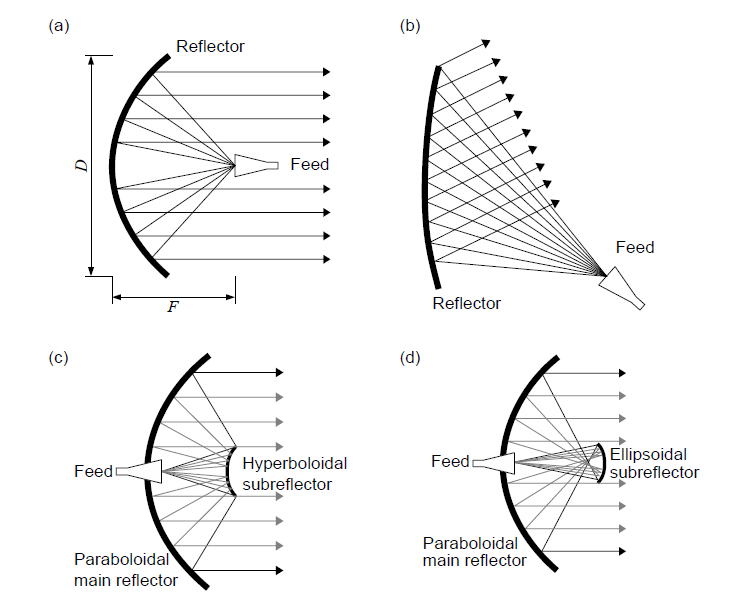
\includegraphics[scale = 0.7]{figures/antennas/reflector/types}
\caption{Reflector antenna configurations: (a) on-focus parabolic reflector; (b) off-axis reflector; (c) Cassegrain reflector; (d) Gregorian reflector \citep{Imbriale2012}}
\label{fig:reflector_types}
\end{figure}

Equation for parabola

\begin{equation}
y=a x^2 , a = \frac{1}{4F}
\end{equation}
\label{eq:para1}

Focal length
\begin{equation}
F=D\frac{1}{4tan(\theta/4)}
\end{equation}
\label{eq:para2}

Length of parabolic segment
\begin{equation}
L=\frac{ln(\sqrt{a^2 D^2 +1}+a D)}{4a}+\frac{D\sqrt{a^2 D^2 +1}}{4}
\end{equation}
\label{eq:para3}

Gain for parabolic reflector

\begin{equation}
G=\eta \frac{4\pi A}{\lambda^2}, A = \frac{\pi D^2}{4}
\end{equation}
\label{eq:para4}

\begin{figure}[H]
\centering 
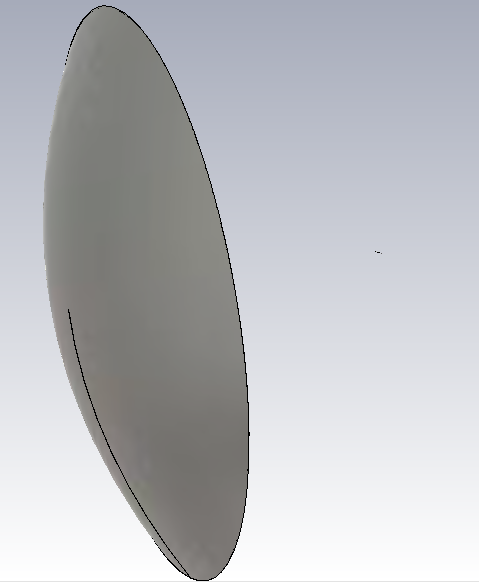
\includegraphics[scale = 0.5]{figures/antennas/reflector/parabola_cst}
\caption{Simulated reflector antenna in CST studio}
\label{fig:para_sim1}
\end{figure}

\begin{figure}[H]
\centering 
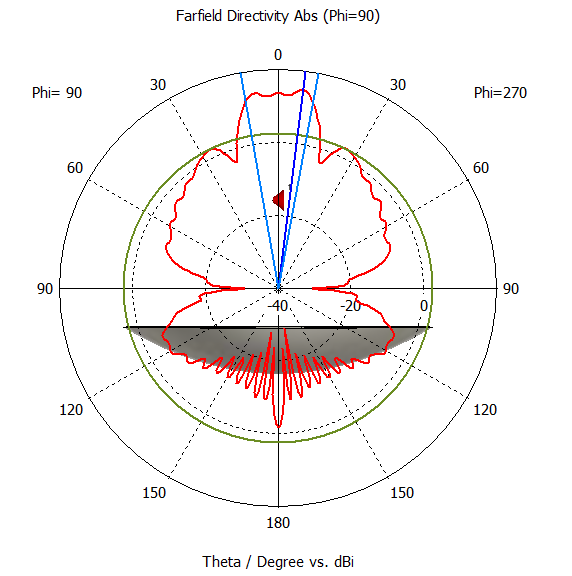
\includegraphics[scale = 0.5]{figures/antennas/reflector/parabola_cst_farfield}
\caption{Farfield of simulated reflector antenna in CST studio}
\label{fig:para_sim2}
\end{figure}



\section{Helical Antennas}
\subsection{Helical antenna with ground plane}

\begin{figure}[H]
\centering 
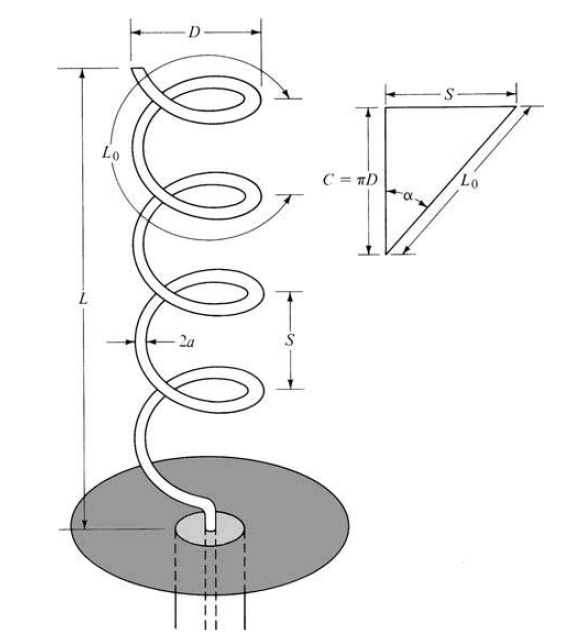
\includegraphics[scale = 0.5]{figures/antennas/helical/helical}
\caption{Helical antenna with ground plane \citep{Balanis2005}}
\label{fig:helical}
\end{figure}

\begin{figure}[H]
\centering 
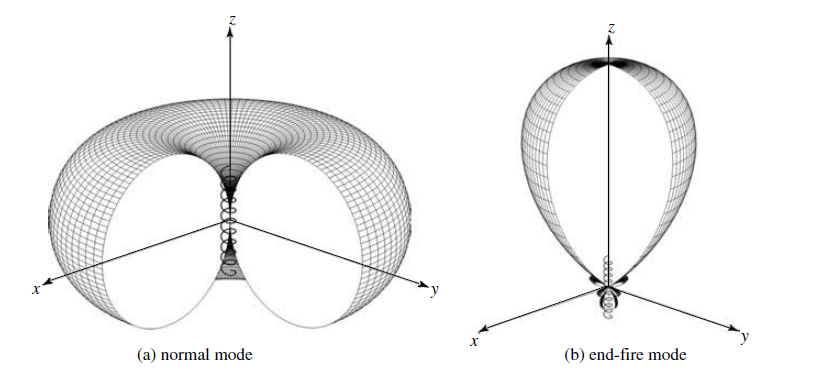
\includegraphics[scale = 0.5]{figures/antennas/helical/modes}
\caption{Farfield for (a) normal mode and (b)end-fire mode \citep{Balanis2005}}
\label{fig:helical_modes}
\end{figure}

A helical antenna is a wire wound in form of a screw and is depicted in figure \ref{fig:helical}. The helical antenna consist of N turns, diameter D and spacing between the turns S and circumference is $C = \pi D$w here the total length is $L = NS$. Normally the helical antenna has a circular ground plane with the diameter $G_d = \frac{3\lambda}{4}$. Another important parameter is the pitch angle $\alpha$ which is the angle formed by a line tangent to the helix wire and a plane perpendicular to the helix axis. The pitch angle is defined by   

\begin{equation}
\alpha = tan^{-1}(\frac{S}{\pi D}) = tan^{-1}(\frac{S}{C})
\end{equation} 

The radiation pattern of the antenna can be varied by controlling the size of its
geometrical properties compared to the wavelength. The input impedance is critically
dependent upon the pitch angle and the size of the conducting wire, especially near the
feed point, and it can be adjusted by controlling their values. The general polarization
of the antenna is elliptical. However circular and linear polarizations can be achieved
over different frequency ranges \citep{Balanis2005}. The helical antenna can operates typically in one of two modes which is
the normal (broadside) and the axial (end-fire) mode see figure \ref{fig:helical_modes}. In end-fire mode a circular polarization is archived if the D and S is large fractions of the wavelength. The design criteria is $\frac{3}{4} < C/\lambda < \frac{4}{3}$ where $C = \lambda$ is optimum. $S = \frac{\lambda}{4}$ this gives a pitch angle between $12^o \leq \alpha \leq 14^o $ and a ground plane at least $G_d = \frac{\lambda}{2}$. Formulas for radiation resistance Half Power Beam Width (HPBW) and reflection coefficient is given by equation \ref{eq:heli1} to \ref{eq:heli4}. The formulas has an accuracy about 20\% the formulas are therefore held up with a simulation at $f = 1GHz$.\\

Directivity
\begin{equation}
D =  15N\frac{C^2 S}{\lambda^3} = 12.7dB
\end{equation}  
\label{eq:heli1}

Half Power Beam Width
\begin{equation}
HPBW = \frac{52\lambda^{3/2} }{C\sqrt{NS}} = 46.5^o
\end{equation}  
\label{eq:heli2}

Impedance of antenna 
\begin{equation}
Z_l = 140\frac{C}{\lambda} = 140\Omega
\end{equation} 
\label{eq:heli3}
 
Reflection coefficient 
\begin{equation}
\Gamma = \frac{Z_l+Z_s}{Z_l-Z_s} = -3.2dB
\end{equation}  
\label{eq:heli4}

The simulation results are depicted in figure \ref{fig:helical_cst} to \ref{fig:helical_farfield}. It can be seen that the simulated results corresponds well with the formulas whit-in 20\% accuracy . 

\begin{figure}[H]
\centering 
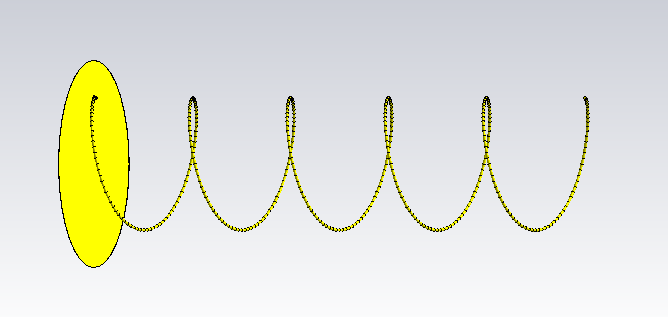
\includegraphics[scale = 0.5]{figures/antennas/helical/helical_cst}
\caption{Simulated helical antenna}
\label{fig:helical_cst}
\end{figure}

\begin{figure}[H]
\centering 
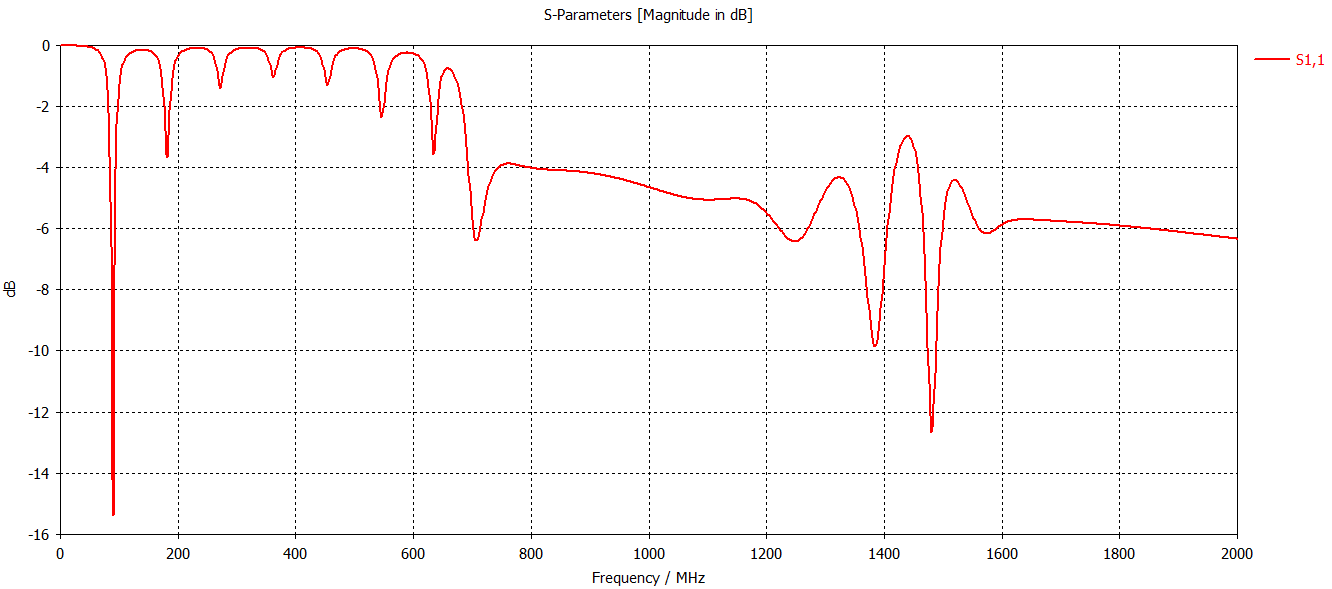
\includegraphics[scale = 0.5]{figures/antennas/helical/helical_cst_s11}
\caption{Reflection coefficient for simulated helical antenna}
\label{fig:helical_s11}
\end{figure}

\begin{figure}[H]
\centering 
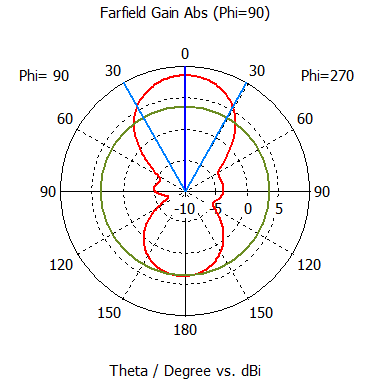
\includegraphics[scale = 0.5]{figures/antennas/helical/helical_cst_farfield}
\caption{Farfield for simulated helical antenna with a maximum directivity a 7.1dB and a HPBW at $58.8^o$}
\label{fig:helical_farfield}
\end{figure}

\subsection{Quadrifilar Helical Antenna}

\begin{figure}[H]
\centering 
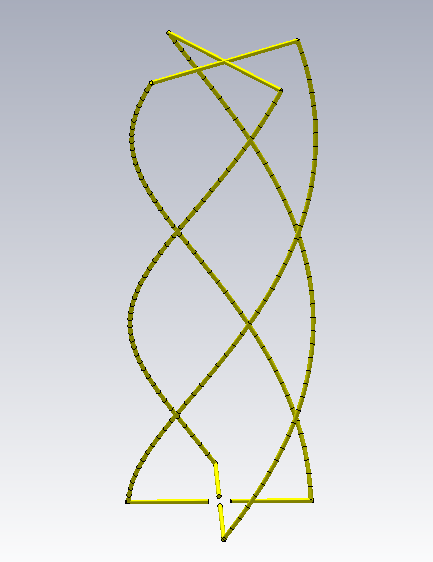
\includegraphics[scale = 0.7]{figures/antennas/qha/qha_6_1mhz}
\caption{QHA with $N=0.6$, $D=80mm$,$L=\frac{\lambda}{2}-D\cdot 0.75$, $f=1GHz$}
\label{fig:QHA1}
\end{figure}

The Quadrifilar Helical Antenna (QHA) (see figure \ref{fig:QHA1}) is an resonant antenna which is typically feed by two ports with a $90^\circ$ phase difference. The antenna has a circular polarization and the size is often smaller than a normal helical antenna. Typically the length of each arm is an integral multiple of the quarter-wavelength. The end of the helix
is open when the integer is odd, while short when the integer is
even \citep{Bai2014}. Despite the typically design the turn ratio, radius, length and feeding topology will affect the radiation pattern and polarization. Another important measure of all helical antennas is the pitch angle which is defined in equation \ref{eq:pitch}.

\begin{equation}
\alpha = tan^{-1}(\frac{S}{\pi D})
\end{equation}
\label{eq:pitch}

Where D is the diameter of the antenna, S is the spacing between the loops and futher N is the number of turns and L is the length of the antenna \citep{Balanis2005}.
\newline
\newline
An QHA has been build and simulated in CST studio. The dimensions are $D=80mm$,$L=\frac{\lambda}{2}-D\cdot 2$, $N=0.6$ at the frequency $f=122.5MHz$ and $\lambda = 2450mm$ with the wire diameter $Wd = 2mm$. The diameter is chosen so the antenna can be stowed in a 10x10x10cm box and the length is calculated so there is a half wavelength between the negative and positive side of a port. The feeding is done using two discrete ports as shoved in figure \ref{fig:QHA2}.  

\begin{figure}[H]
\centering 
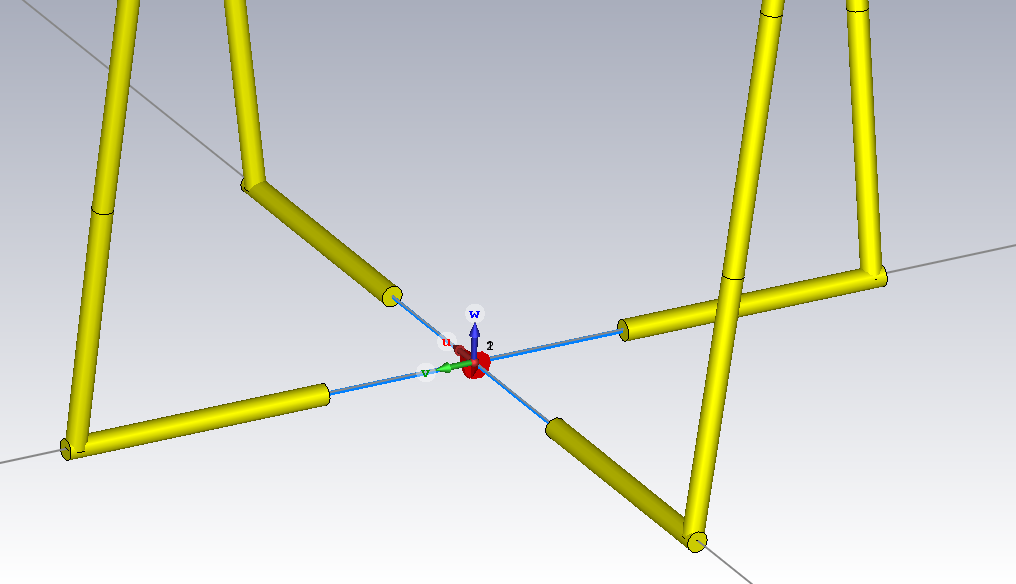
\includegraphics[scale = 0.4]{figures/antennas/qha/qha_6_feeding}
\caption{Feeding of the QHA for 122.5MHz using discrete ports}
\label{fig:QHA2}
\end{figure}
 
The QHA has been simulated and the results shows, that the antenna is matched to 131MHz even thou the S11 parameter at this frequency is only -2dB, see figure \ref{fig:QHA_S11}. The error is caused by the gap between the ports in the bottom and the extra length caused by the turn of N. It can be seen that the antenna also radiates at multiply of the match frequency and that the lowest return-loss is obtained at 4 times the frequency which gives 524MHz. The farfields for the frequencies 131,262 and 393MHz are shown in figure \ref{fig:QHA_ff_131}, \ref{fig:QHA_ff_262} and \ref{fig:QHA_ff_393}, where port 1 is fed with a positive phase at $90^\circ$. It is seen that the farfield not surprisingly changes with the frequency. The farfield suited best for tracking of ADS-B signals is the one in figure \ref{fig:QHA_ff_131}. \todo[inline,color=orange]{write someting about the earth curvature and why?}.      

\begin{figure}[H]
\centering 
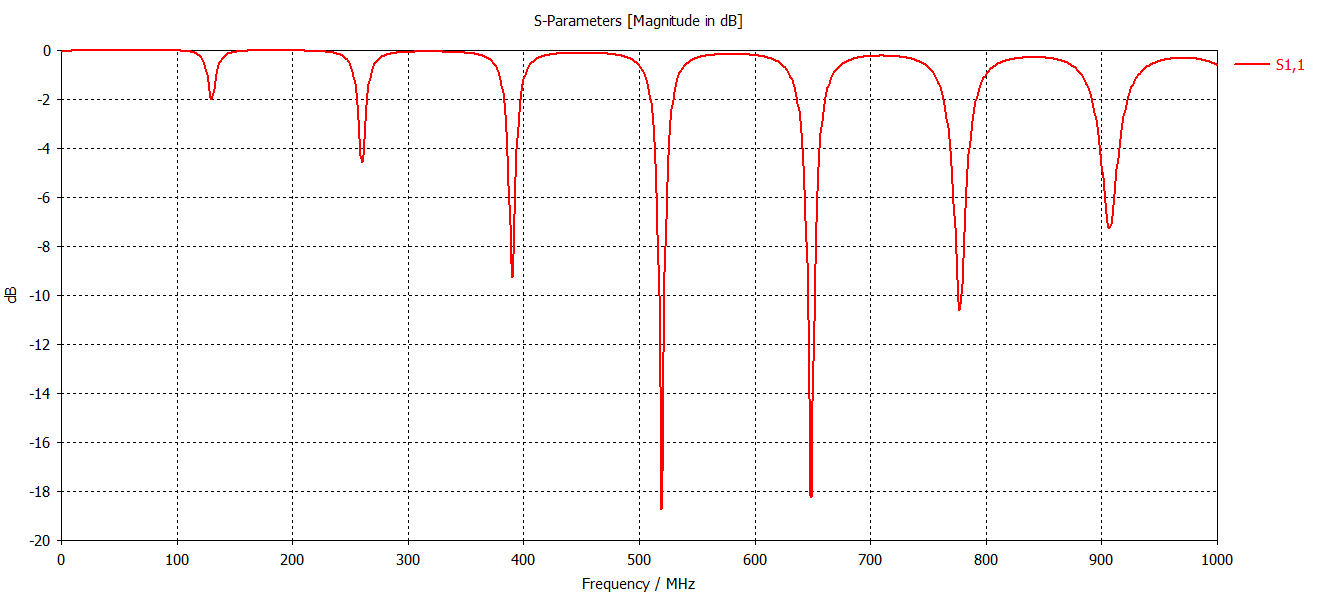
\includegraphics[scale = 0.5]{figures/antennas/qha/qha_6_S11}
\caption{S11 parameter of the QHA for 122.5MHz}
\label{fig:QHA_S11}
\end{figure}

\begin{figure}[H]
\centering 
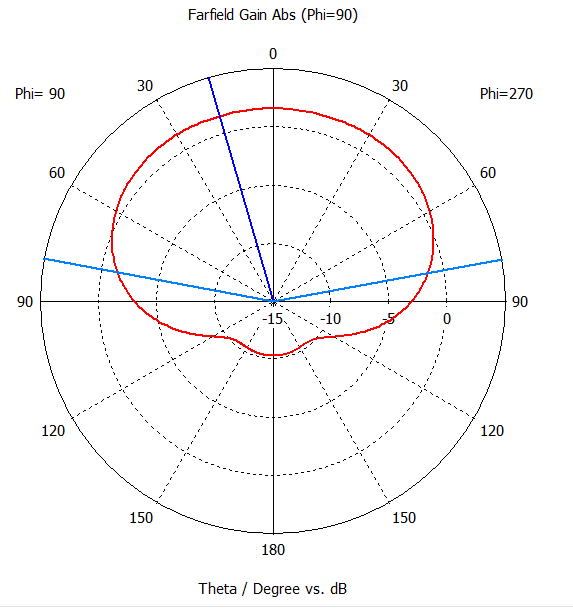
\includegraphics[scale = 0.5]{figures/antennas/qha/qha_6_ff_131}
\caption{Simulated farfield at 131MHz}
\label{fig:QHA_ff_131}
\end{figure}

\begin{figure}[H]
\centering 
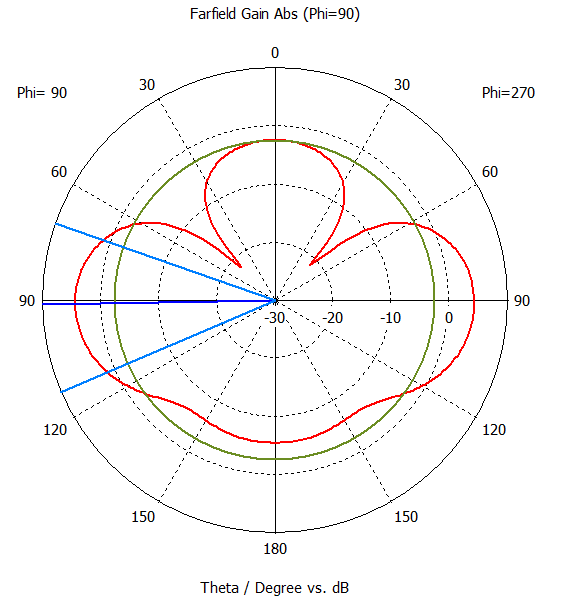
\includegraphics[scale = 0.5]{figures/antennas/qha/qha_6_ff_262}
\caption{Simulated farfield at 262MHz}
\label{fig:QHA_ff_262}
\end{figure}

\begin{figure}[H]
\centering 
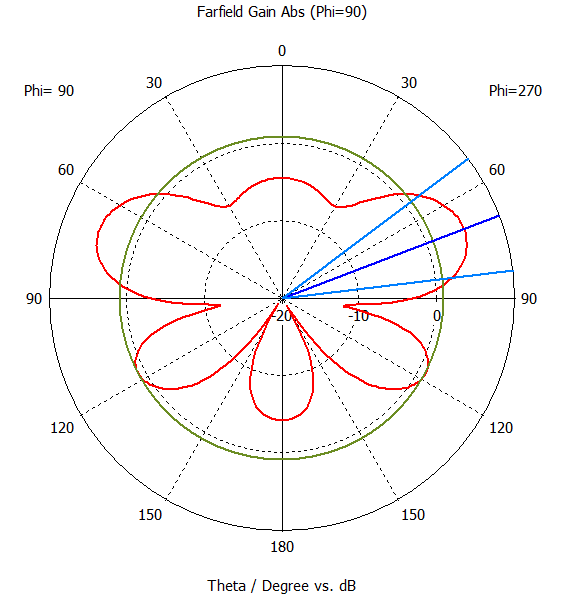
\includegraphics[scale = 0.5]{figures/antennas/qha/qha_6_ff_393}
\caption{Simulated farfield at 393MHz}
\label{fig:QHA_ff_393}
\end{figure}

%%%%%%%%%%%%%%%%%%%%%%%%%%%%%%%%%%%%%%%%%%%%%%%%%%%%%%%%%%%%%%%%%%%%%%%%%%%%%%%%%%%%% Feeding %%%%%%%%%%%%%%%%%%%%%%%%%%%%%%%%%%%%%%%%%%%%%
\subsubsection{Feeding methods}
In figure \ref{fig:QHA2} the feeding of the QHA is done using two discrete ports. When port 1 is fed with a positive phase at $90^\circ$ the QHA will have it's maximum radiation in the forward direction. If the port instead is fed with a negative phase at $90^\circ$ then the QHA will have it's maximum radiation in the backward direction. Other phases will result in non-uniform radiation patterns with one ore more peaks in the azimuth axis. It is easy to believe that it is possible to connect two of the arms of the QHA to a common ground and feed the one port with a phase difference at $90^\circ$ using a $1/4 \lambda $ transmission-line and the other directly from the source depicted in figure \ref{fig:QHA_common}. But this will not work since the geometry of the QHA will change from an electrically perspective. The shortening of the two grounds will affect the flow of the current resulting of only a pattern difference of $45^\circ$ in the farfield which then makes it impossible to archive a omnidirectional radiation pattern and circular polarization. To overcome this is has been shown in \citep{Bai2014} that it is possible to use a feeding network consisting of one second-iteration Moore $180^\circ$ hybrid coupler and two second-iteration Sierpinski $90^\circ$ hybrid couplers. It has also been showen in \citep{Yang2014} that a broadband feed network can be done using an wilkinson powerdivider and broadband $90^\circ$ phase shifters.     

\begin{figure}[H]
\centering 
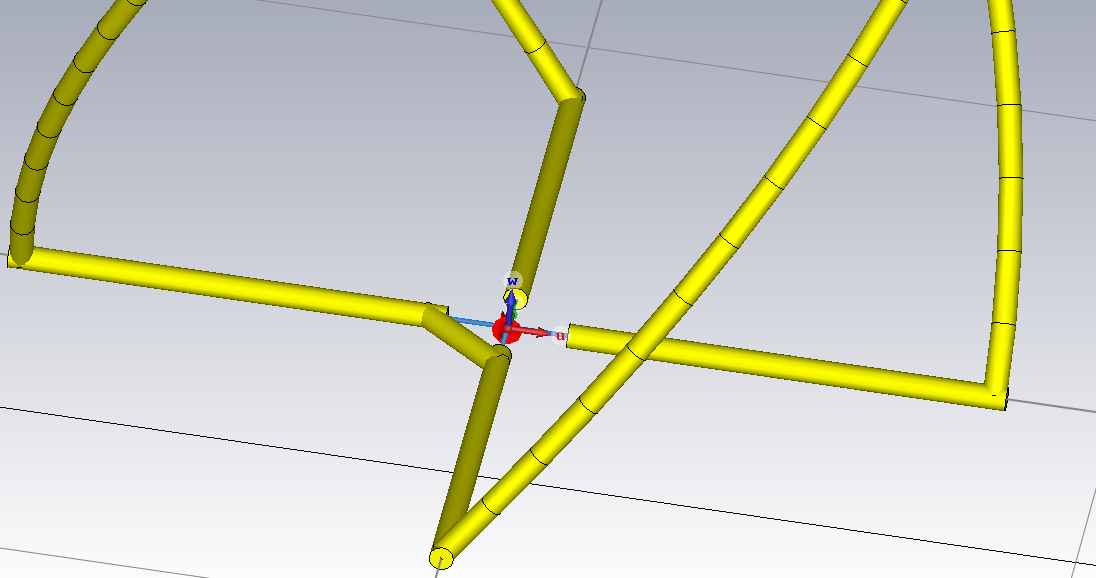
\includegraphics[scale = 0.3]{figures/antennas/qha/qha_6_common_gnd}
\caption{Common GND for the QHA}
\label{fig:QHA_common}
\end{figure}

\subsubsection{Wideband QHA}
As shown previously a QHA in its basic form radiates only at a narrow frequency band. For the S-parameters in figure \ref{fig:QHA_S11} it is seen that at 131MHz the return loss is about -2dB which results in an efficiency at only -5dB. This can be improved using a match network, but the antenna still needs to be a radiating element and therefore the matching can only improve the return-loss and not the bandwidth \citep{Iyver2010}. Therefore some modifications needs to be done at the QHA to improve the bandwith.     

%%%%%%%%%%%%%%%%%%%%%%%%%%%%%%%%%%%%%%%%%%%%%%%%%%%%%%%%%%%%%%%%%%%%%%%%%%%%%%%%%%%%%%%%%%%%%%%%%%%%%%%%%%%%%%%%%%%%%%%%%%%%%%%%%% 


\section{Spiral antennas}


\subsection{Conical Log-Spiral antenna}

\begin{figure}[H]
\centering 
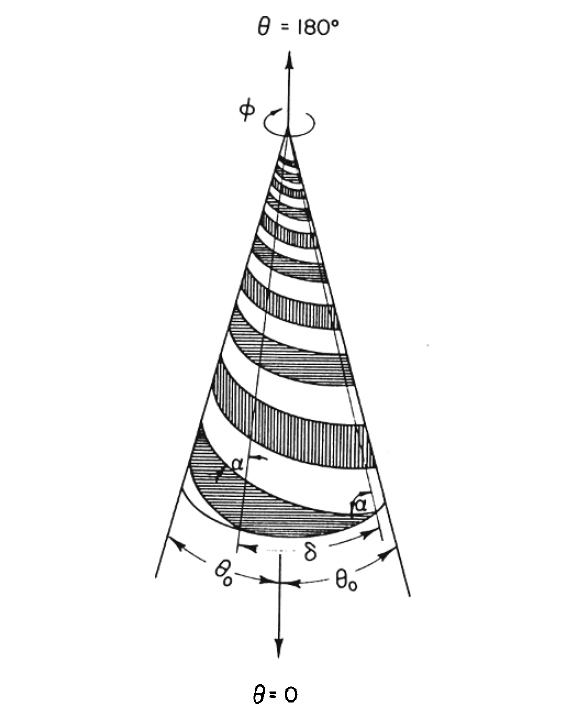
\includegraphics[scale = 0.5]{figures/antennas/spiral/conical_spiral}
\caption{Conical spiral antenna \citep{Rumsey1966}}
\label{fig:con_spi}
\end{figure}


The balanced two arm Conical Log-Spiral Antenna (CLSA) depicted in figure \ref{fig:con_spi} is a derivative of planar spiral antennas which all are frequency independent because the geometry is only described by angles \citep{Balanis2005}. The CLSA consist of two metal strips on the surface of a cone, whose shapes are defined by the equiangular spiral of equation \ref{eq:spiral} \citep{Rumsey1966}.

\begin{equation}
r = e^{\alpha\phi sin(\theta_0)}
\end{equation}
\label{eq:spiral} 

The angle $\alpha$ between the radius and the tangent to the spiral is $cot^{-1}(\alpha)$ and because of the spiral $\theta_0 = 90^\circ$. The CSA do also have circular polarization which makes it usable for satellite communication. 



%%%%%%%%%%%%%%%%%%%%%%%%%%%%%%%%%%%%%%%%%%%%%%%%%%%%%%%%%%%%%%%%%%%%%%%%%%%%%%%%%%%%%%%%%%%%%%%%%%%%%%%%%%%%%%%%%%%%%%%%%%%%%%

\section{Horn antennas}
\section{Printed antennas}










    



   
\chapter{Basic Theory}\label{ch:2}

\section{Non-linearity}

\begin{figure}[H]
\centering 
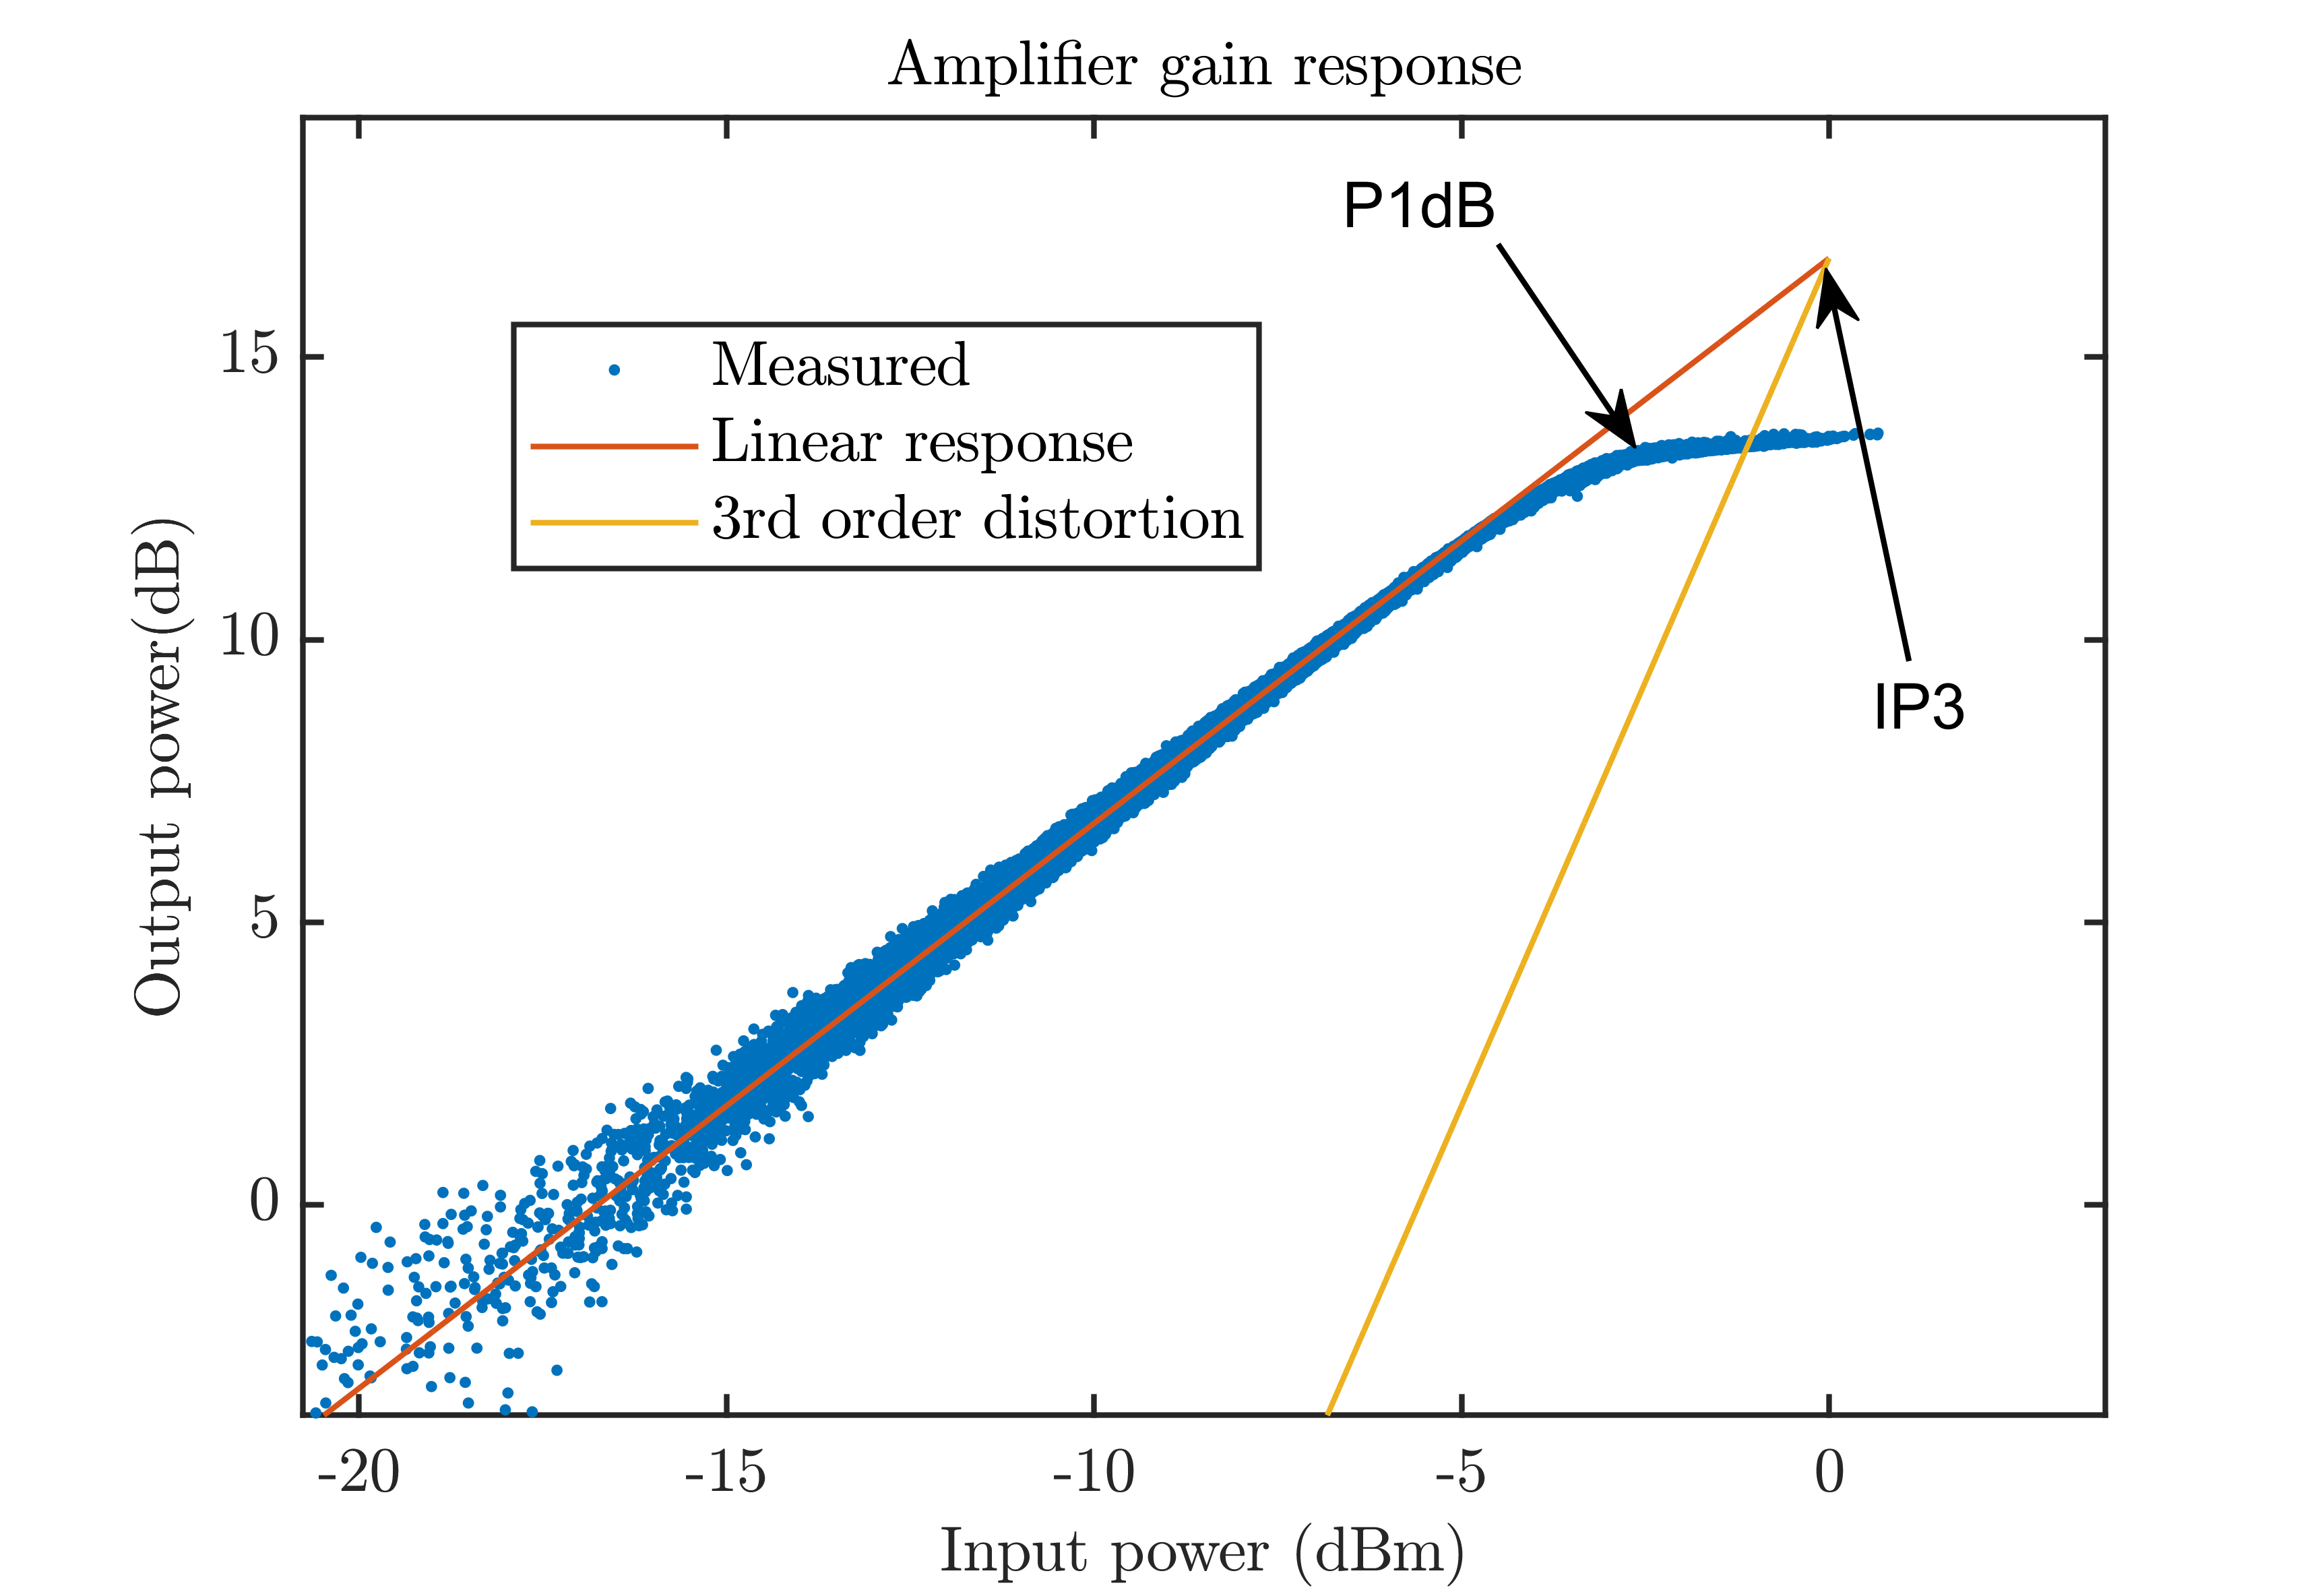
\includegraphics[scale = 0.8]{figures/ch1/amp_lin.png}
\caption{Amplifier non-linearity}
\label{fig:amp_lin}
\end{figure} 

An ideal power amplifier has an linear response over all frequencies and input power. This is depicted in \ref{fig:amp_lin} as Linear response. Unfortunately this is not true and therefore a measurement of a power amplifier has been done. The measurement shows that the amplifier at some level can be assumed linear, but at a point the amplifier will saturate due to the supply voltage and the gain will compress. The point where there is 1dB from the linear response to the real response is called the 1dB compression point (P1dB) which is also depicted in  figure \ref{fig_amp_lin}. The non-linear gain response causes a distortion at the output which can be described by equation \ref{eq:dest} \citep{NI}. If a input-signal using two tones is considered then there will be a difference and a sum of the frequencies presented at the output which is caused by the cubic term in equation \ref{eq:dest2}.

\begin{equation} \label{eq:dest}
V_{out} = a_0 + a_1 V_{in} + a_2 V_{in}^2 + a_3 V_{in}^3 + a_4 V_{in}^4 + ... 
\end{equation}

Where $V_{out}$ is the output signal from the amplifier, $a_1, a_2 ,a_3..$ is coefficients describing the ratio of the distortion and $V_{in}$ is the input signal. If a single tone input is presented, then the output will consist of purely odd and even harmonic distortion. 

\begin{equation}\label{eq:dest1}
V_{in} = sin(\omega_1 t) + sin(\omega_2 t)
\end{equation} 

\begin{equation} \label{eq:dest2}
V_{out} = a_0 + a_1 (sin(\omega_1 t) + sin(\omega_2 t)) + a_2 (sin(\omega_1 t) + sin(\omega_2 t))^2 + a_3 (sin(\omega_1 t) + sin(\omega_2 t))^3 + ... 
\end{equation}

This is also called Two-Tone Third-Order Intermodulation Distortion and is also depicted in figure \ref{fig:amp_lin} as 3rd order distortion with a slope of 3:1. It can bee seen that when the output power increases then the 3rd order distortion increases 3 times. A measurement of this is called the third-order-intercept-point (IP3 or TOI). However, the intercept point it not directly measurable since the amplifier reaches compression way before. It can bee seen from figure \ref{fig:amp_psd} that the distorted component are spaced too close in frequency to be effectively filtered. This will cause distortion into nearby channels and is measured as Adjacent Channel Power Ratio (ACPR).

\begin{figure}[H]
\centering 
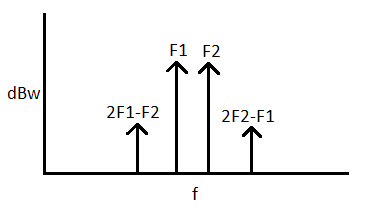
\includegraphics[scale = 0.7]{figures/ch1/amp_psd.png}
\caption{Two-Tone Third-Order Intermodulation Distortion}
\label{fig:amp_psd}
\end{figure}

%%%%%%%%%%%%%%%%%%%%%%%%%%%%%%%%%%%%%%%%%%%%%%%%%%%%%%%%%%%%%%%%%%%%%%%%%%%%%%%%%%%%%%%%%%%%%%%%%%%%%%%%%%%%%%%%%%%%
\subsubsection{Distortion due to non-linearity}

\begin{figure}[H]
\centering 
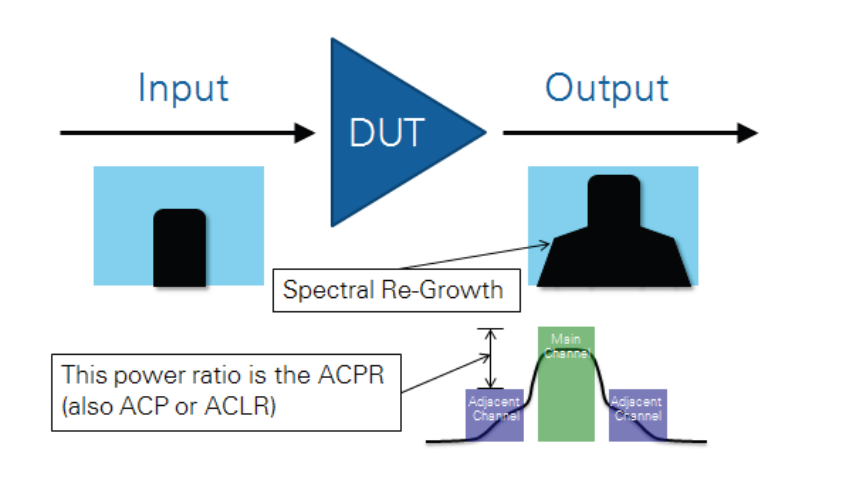
\includegraphics[scale = 0.5]{figures/ch1/acpr.png}
\caption{Graphical Depiction of ACPR in the frequency domain \citep{NI}}
\label{fig:acpr}
\end{figure}

Due to the non-linearity of the PA described before, spectral regrowth will occur which will affect nearby channels. The Adjacent Channel Power Ratio (ACPR) is a measure of the power of the distortion components, caused by the non-linearity of the PA, that are leaked into the adjacent channel see figure \ref{fig:acpr}. The formula for the ACPR is given by equation \ref{eq:acpr} and is used after a Fourier transform has been performed at the output signal of the PA.

\begin{equation} \label{eq:acpr}
	ACPR = \frac{\int_{adjch}^{} |Y(f)|^2 df }{\int_{mainch}^{} |Y(f)|^2 df}
\end{equation}   

Where $Y(f)$ is the Fourier transform of the signal, adjch is the adjacent-channel and mainch is the main-channel. 

\begin{figure}[H]
\centering 
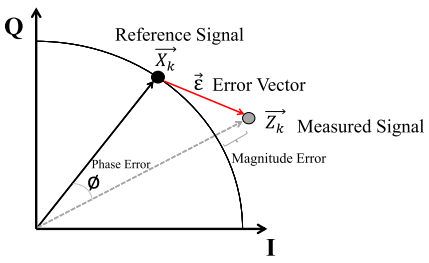
\includegraphics[scale = 0.8]{figures/ch1/evm.png}
\caption{Graphical view of the EVM}
\label{fig:evm}
\end{figure}
  
Another measure of the error is the Error Vector Measurement (EVM) or  Relative Constellation Error (RCE) which both is a measure of the error due to the constellations points in a IQ plot. If a signal is sent through an amplifier with a given IQ value, then the amplifier will distort those IQ values. The EVM and RCE is a measure of the power of the error vector divided by the power of the reference vector. \citep{ali2016}

\begin{equation} \label{eq:evm}
	EVM = \frac{P_{error}}{P_{reference}} = \frac{E[|z(t)-x(t)|^2]}{E[|x(t)^2|]}
\end{equation}  
 
%\begin{figure}[H]
%\centering 
%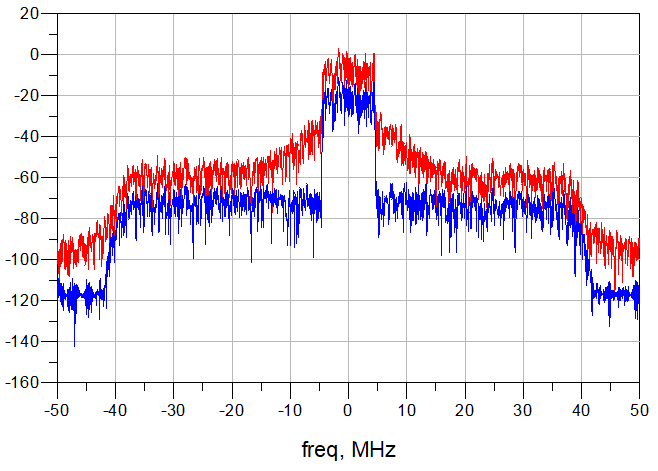
\includegraphics[scale = 0.5]{figures/ch1/ads_nonlin_dest.png}
%\caption{Destortion simulated in ADS, where blue is input-signal and red is output-signal. The simulation is made %with a single amplifier connected to a $50\Omega$ resistor. It is clearly that the output-signal is distorted. The %ACPR becomes -45dB with a BW at 10MHZ}
%\label{fig:pre_cons}
%\end{figure}


\section{AM/AM and AM/PM distortion}
If the input signal to the PA is modelled as equation \ref{eq:amam1}

\begin{equation}\label{eq:amam1}
x(t) = a(t)e^{j\phi(t)}
\end{equation}

Where $a(t)$ is the envelope of the signal and $e^{j\phi(t)}$ is the phase of the input signal. Then the distorted output of the amplifier will be that of equation \ref{eq:amam2} where $g(t)$ is the amplitude distortion and $f(t)$ is the phase distortion also called Amplitude to Amplitude (AM/AM) and Amplitude to Phase (AM/PM) distortion. AM/AM distortion can be defined as the deviation from the constant gain when PA is
operated in compression region. On the other hand, the increased phase change at compression
region can be termed as AM/PM distortion.In presence of wideband signals having non constant amplitude, PA behaves as nonlinear system and exhibits two types of non-linearities \citep{guo2015} which is static distortion and memory effects.  

\begin{equation}\label{eq:amam2}
y(t) = g(a(t))e^{j\phi(t)+f(a(t))}
\end{equation}

\subsubsection{Memory effects}

\begin{figure}[H]
\centering 
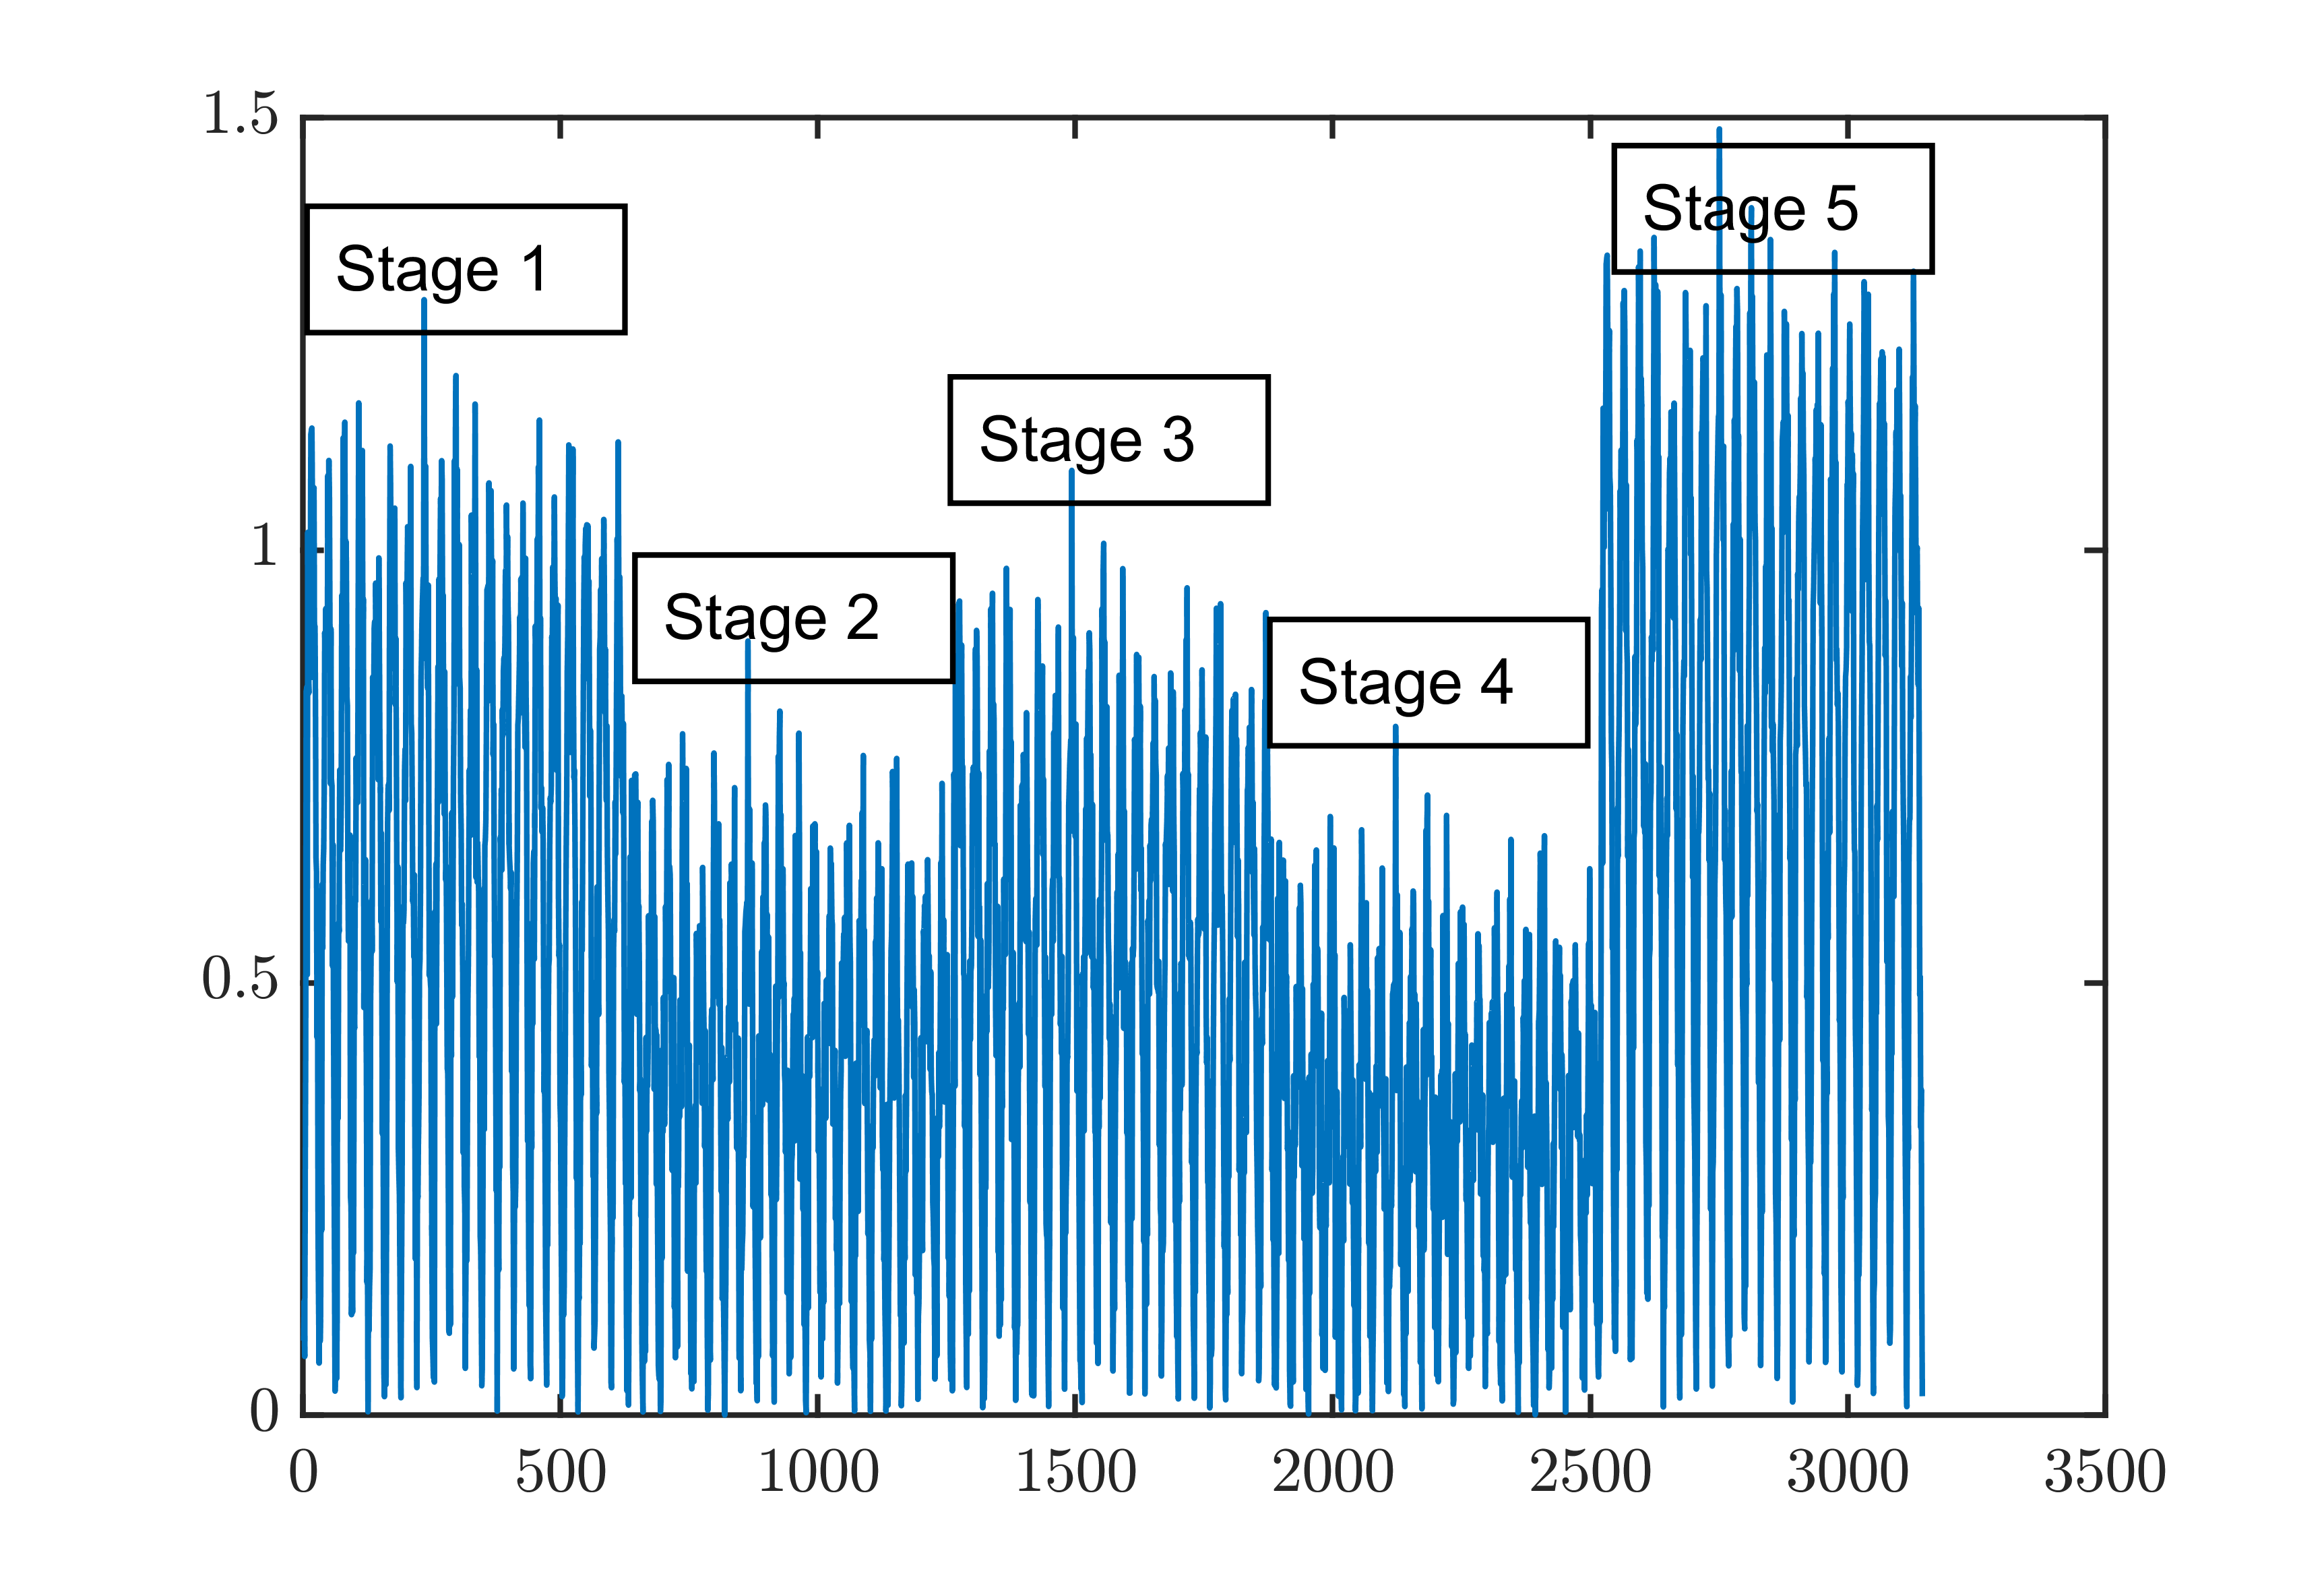
\includegraphics[scale = 0.7]{figures/ch1/amplitude.png}
\caption{Example of amplitude changes at the input of a PA }
\label{fig:mem_amp}
\end{figure}


In modern communication systems, the input power to the PA may be adjusted corresponding to the needs by the network. This makes a suddenly increase or decrease in the power as depicted in figure \ref{fig:mem_amp} which makes the PA work in the transient stage \citep{liu2007}. The transient stage is where the power suddenly increases or decreases to another mean power, whereas the steady state is when the PA operates under stable conditions where the mean power is constant. When the PA is operated in steady state under a high mean power, the amplifier will begin to dissipate heat. This will cause the internal transistors to operate under a hot state where the characteristic of the transistors will change due to a colder state. If the mean power suddenly is decreased the amplifier will still be hot, but with time the amplifier will cool down and the characteristic will change. This can be called slow memory effects whereas fast memory effects is when the amplifier is driven in its steady state and the parasitics of the components distort the signal. Also antennas at the output of the amplifier has an important role specially if several antennas are connected to form an array. The electrical field will couple to each other and cause fields that will affect the memory effects in the system. 


\section{Efficiency}
An important measure of an amplifier is its efficiency, specially when the amplifier is located in a battery powered application. The efficiency of a amplifier is given by equation \ref{eq:effi}

\begin{equation} \label{eq:effi}
\eta = \frac{P_{out}}{P_{amplifier}+P_{out}} = \frac{P_{out}}{P_{DC}}
\end{equation}

Where $P_{out}$ is output power from the amplifier, $P_{amplifier}$ is power dissipated in the amplifier and $P_{DC}$ is the power DC consumption. A more common way to express the efficiency is in terms of power added efficiency (PAE) which is a measure of the difference of power between the output and the input signals versus the DC power consumption.

\begin{equation} \label{eq:effi2}
PAE = \frac{P_{out}-P_{in}}{P_{DC}}
\end{equation}
 


%%%%%%%%%%%%%%%%%%%%%%%%%%%%%%%%%%%%%%%%%%%%%%%%%%%%%%%%%%%%%%%%%%%%%%%%%%%%%%%%%%%%%%%%%%%%%%%%%%%%%%%%%%%%%%%%%%%%
\section{Antenna Diversity and MIMO}

\begin{figure}[H]
\centering 
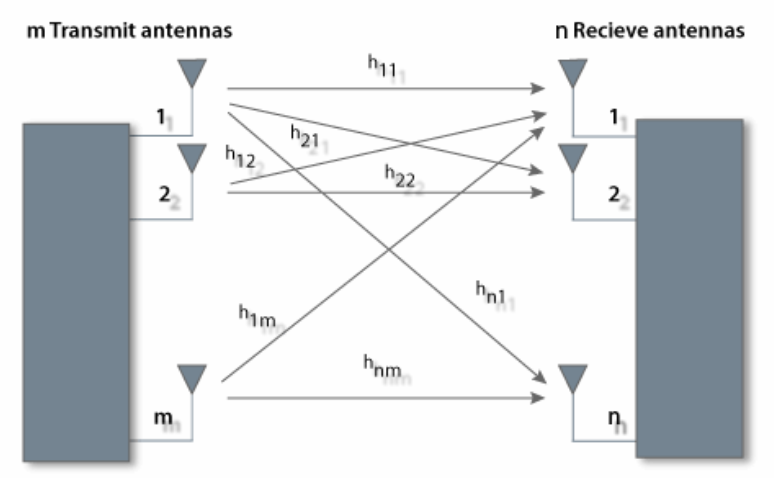
\includegraphics[scale = 0.4]{figures/ch1/mimo.png}
\caption{Concept of MIMO \citep{silvus2019}}
\label{fig:mimo}
\end{figure}

MIMO (Multiple Input Multiple Output) systems are systems with Multiple Element Antennas at both link ends. The antenna elements of a MIMO system can be used for four different purposes: beamforming, diversity, interference suppression, and spatial multiplexing which is transmission of several data streams in parallel that allows improvement of capacity.\citep{molisch2011} A MIMO system is modelled as in equation \ref{eq:mimo} and is also depicted in figure \ref{fig:mimo}.

\begin{equation}\label{eq:mimo}
\textbf{y = Hx+n}
\end{equation}  

Where \textbf{y} is the received vector, \textbf{H} is the channel matrix, \textbf{x} is the transmitted vector and \textbf{n} is noise. The principle of MIMO is to ensure that the same information reaches the receiver on several
statistically independent channels. In MIMO systems, several transmits paths is archived by use of several antennas, which gives a spatial separation if they are separated enough to give a correlation factor $\rho$ that is below $0.5 - 0.7$ \citep{molisch2011}. The formula for the envelope correlation factor between two antennas is given by equation \ref{eq:corr_fac}. The formula assumes that the WSSUS (Wide-Sense Stationary Uncorrelated Scattering) model is valid, no LOS exists, the power delay profile has an exponential shape, the incident power is isotropically distributed in azimuth and only propagates in the horizontal plane, and an omnidirectional antenna is used.

\begin{eqnarray} \label{eq:corr_fac}
\rho = \frac{J_0^2( k_0 v \tau)}{1+(2\pi)^2 S_\tau^2(f_2 - f_1)^2 }
\end{eqnarray}      

Where $J_0$ is the Bessel function of the first kind and $S_\tau$ is the delay-spread of the channels. If the correlation between two antennas is investigated for the same frequency, then the formula can be rewritten as equation \ref{eq:corr_fac_re} because $f2-f1=0$.

\begin{eqnarray} \label{eq:corr_fac_re}
\rho = J_0^2( 2\pi d)^{-1}
\end{eqnarray} 

Where $d$ is the element spacing given in wavelengths. A plot of this can bee seen in figure \ref{fig:correlation}.

\begin{figure}[H]
\centering 
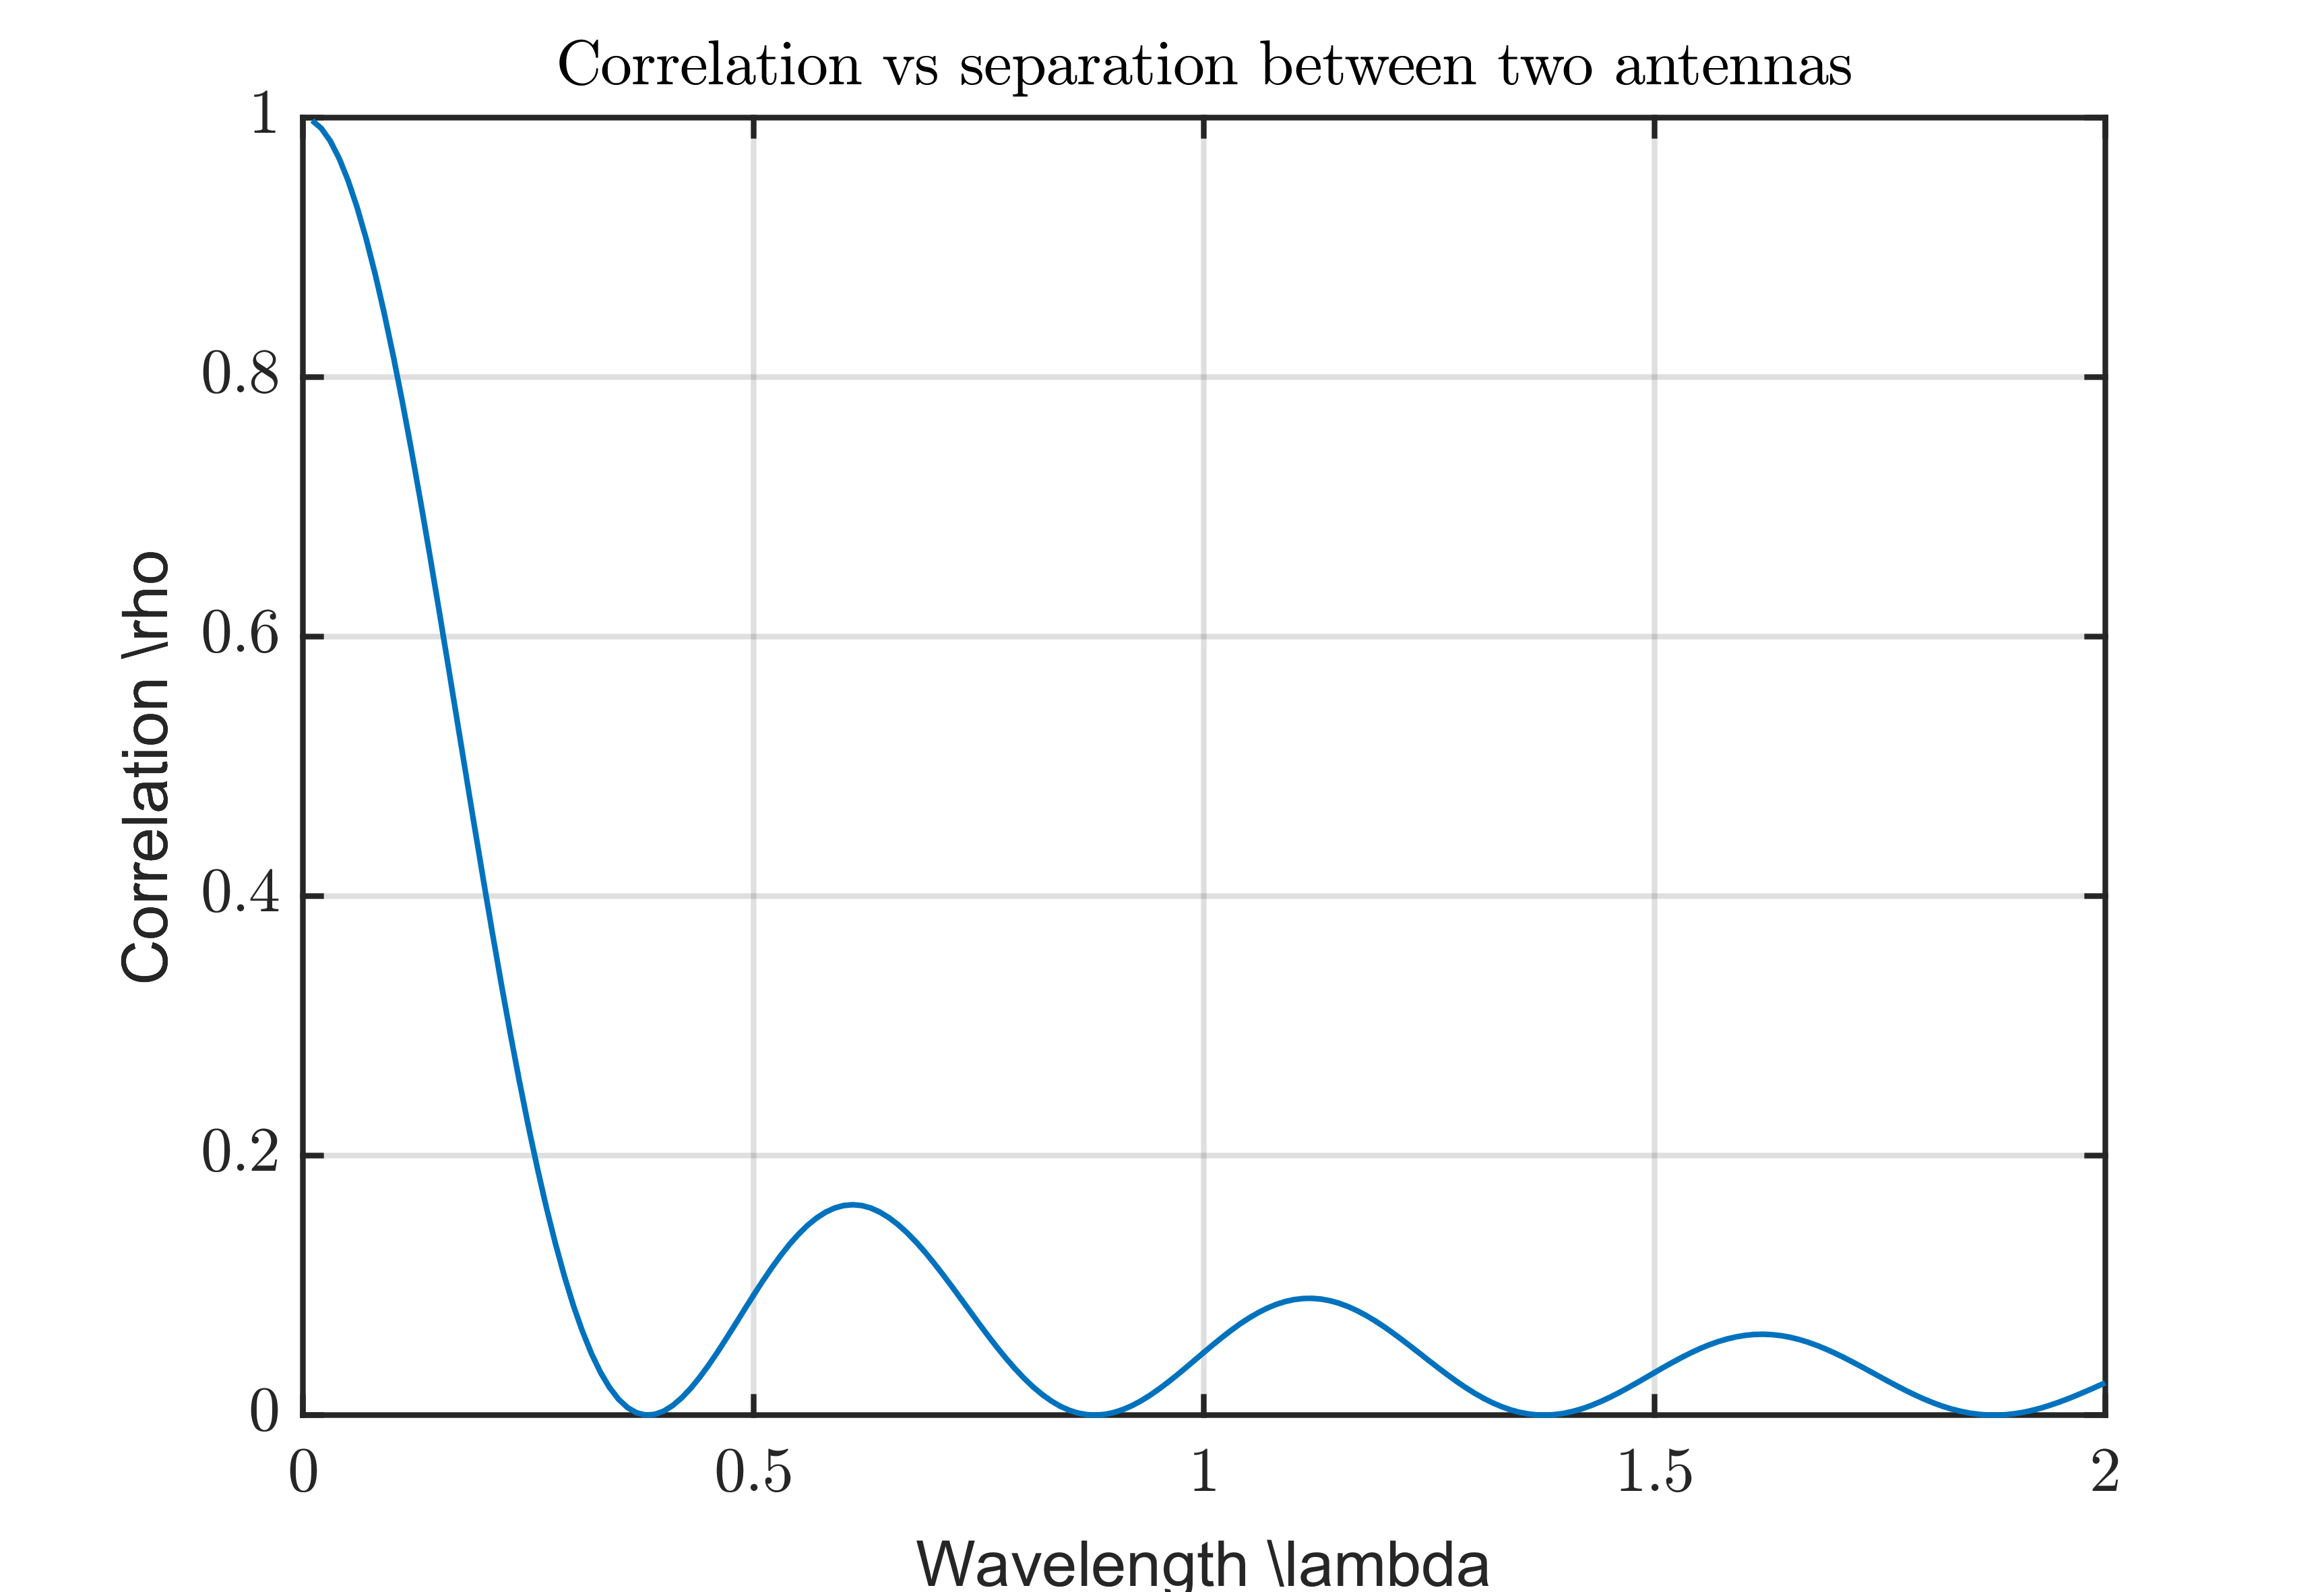
\includegraphics[scale = 0.7]{figures/ch1/correlation.png}
\caption{Correlation factor for two antennas versus distance}
\label{fig:correlation}
\end{figure}

Another method to calculate the correlation factor is to use measured or simulated S-parameters as shown in equation \ref{eq:spar_corr} \citep{wang2011} where k is the propagation constant and d the distance in meters. 

\begin{equation} \label{eq:spar_corr}
\rho = \frac{A+B J_0(kd)}{B+A J_0(kd)}
\end{equation}

\begin{equation} 
A = -2Re(S_{12}^*(1-S_{11}))
\end{equation}

\begin{equation} 
B = |1-S_{11}|^2 + |S_{12}|^2
\end{equation}

Because of the correlation factor all the measurements in this report will be done with an Tx antenna spacing at $d = [0.1 \ 0.2 \ 0.3 \ 0.4 \ 0.5 \ 0.6]^T \lambda$. It is assumed that for most of the cases an antenna array is spaced with $0.5\lambda$ between the elements. 
%%%%%%%%%%%%%%%%%%%%%%%%%%%%%%%%%%%%%%%%%%%%%%%%%%%%%%%%%%%%%%%%%%%%%%%%%%%%%%%%%%%%%%%%%%%%%%%%%%%%%%%%%%%%%%%%%%%

\section{Array factor}
When several antennas are spaced relatively close to each other it is called an antenna array. If the antennas are isotopic and are spaced with a half wavelength then the array will radiate twice the energy in the direction perpendicular to the array, thou the gain along the array will become zero. A mathematical expression of this is called the array factor (AF).

\begin{equation}
AF = \sum_{n=1}^{N} e^{(n J 2\pi d \cos(\alpha)+JB(n))}
\end{equation}

Where N is number of antennas in the array, d is the distance between the antennas, $\alpha$ is the azimuth angle from $0..2\pi$ and B is the feeding phase of a single antenna. In figure \ref{fig:af_2ant} and \ref{fig:af_4ant} the array factor for 2 and 4 antennas spaced  $d = [0.1 \ 0.2 \ 0.3 \ 0.4 \ 0.5 \ 0.6]^T \lambda$ are plotted respectively. It is seen that the energy doubles in the $90^\circ$ for all distances in figure \ref{fig:af_2ant} while it becomes 4 times greater in figure \ref{fig:af_4ant}. This seems also to correspond with the meausrement in chapter \ref{ch:ant_meas}.   


\begin{figure}[H]
\centering 
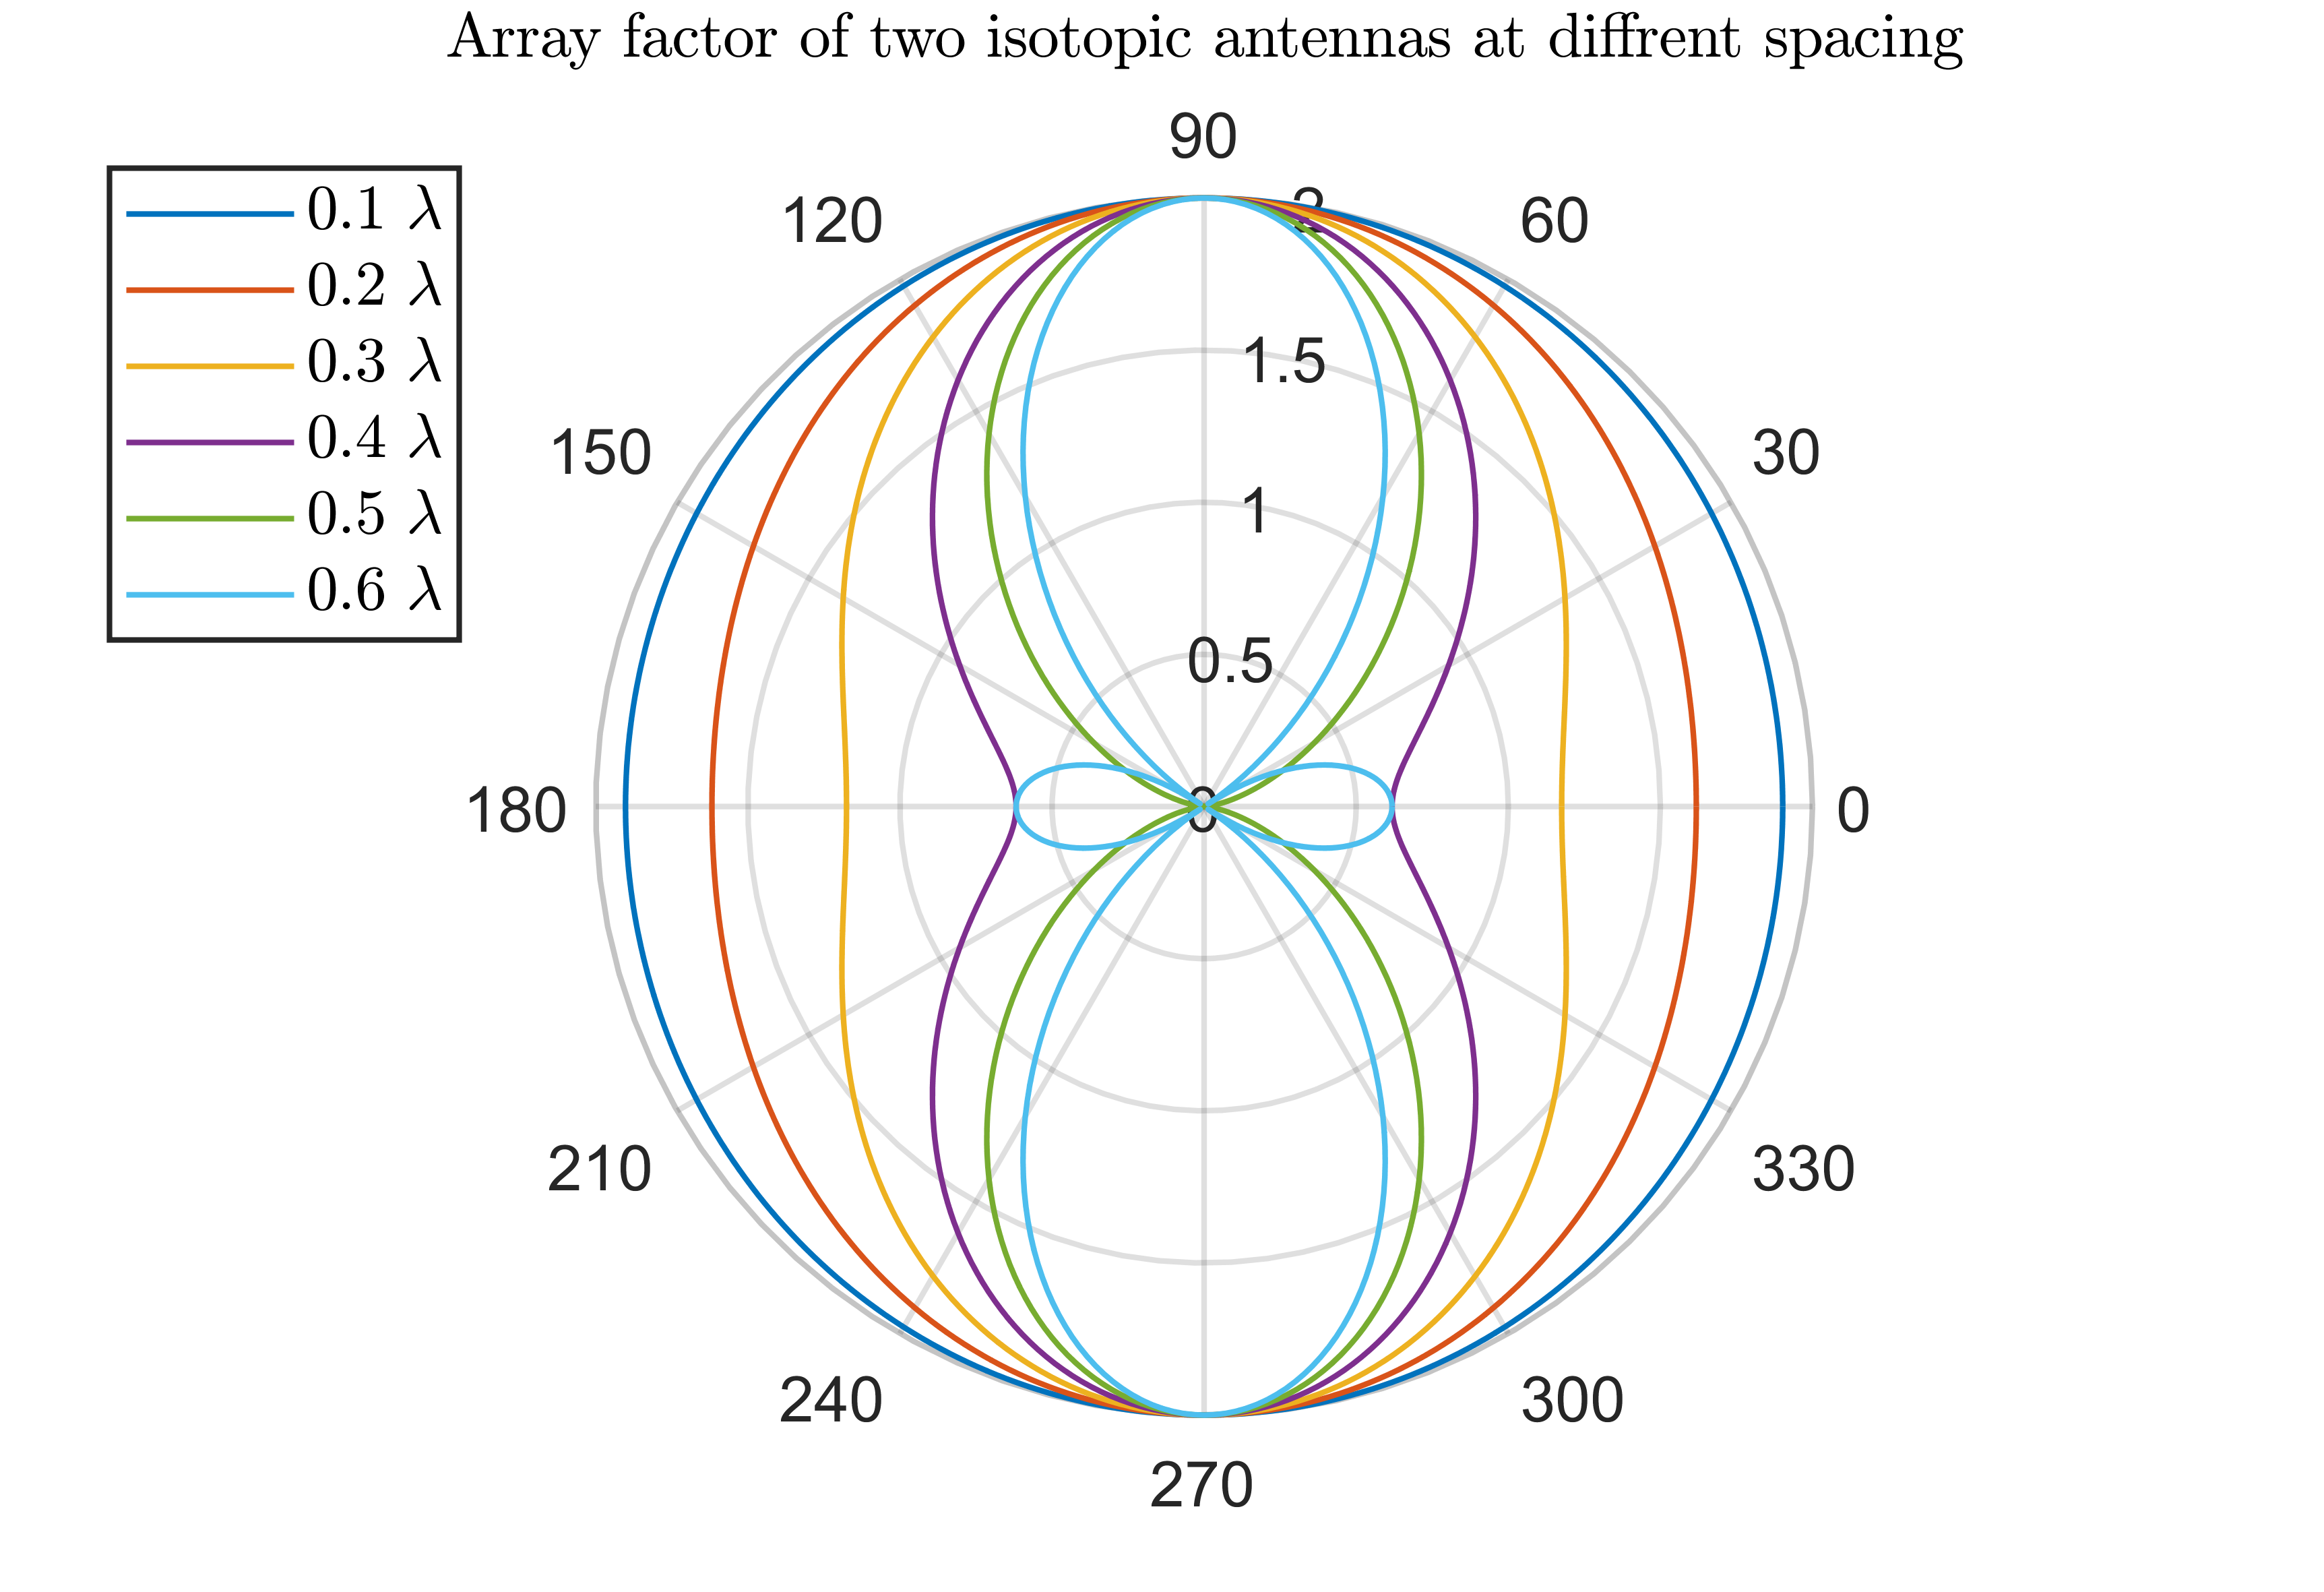
\includegraphics[scale = 0.7]{figures/measurement/af_2ant.png}
\caption{Array factor of two antennas with diffrent spacing}
\label{fig:af_2ant}
\end{figure}


\begin{figure}[H]
\centering 
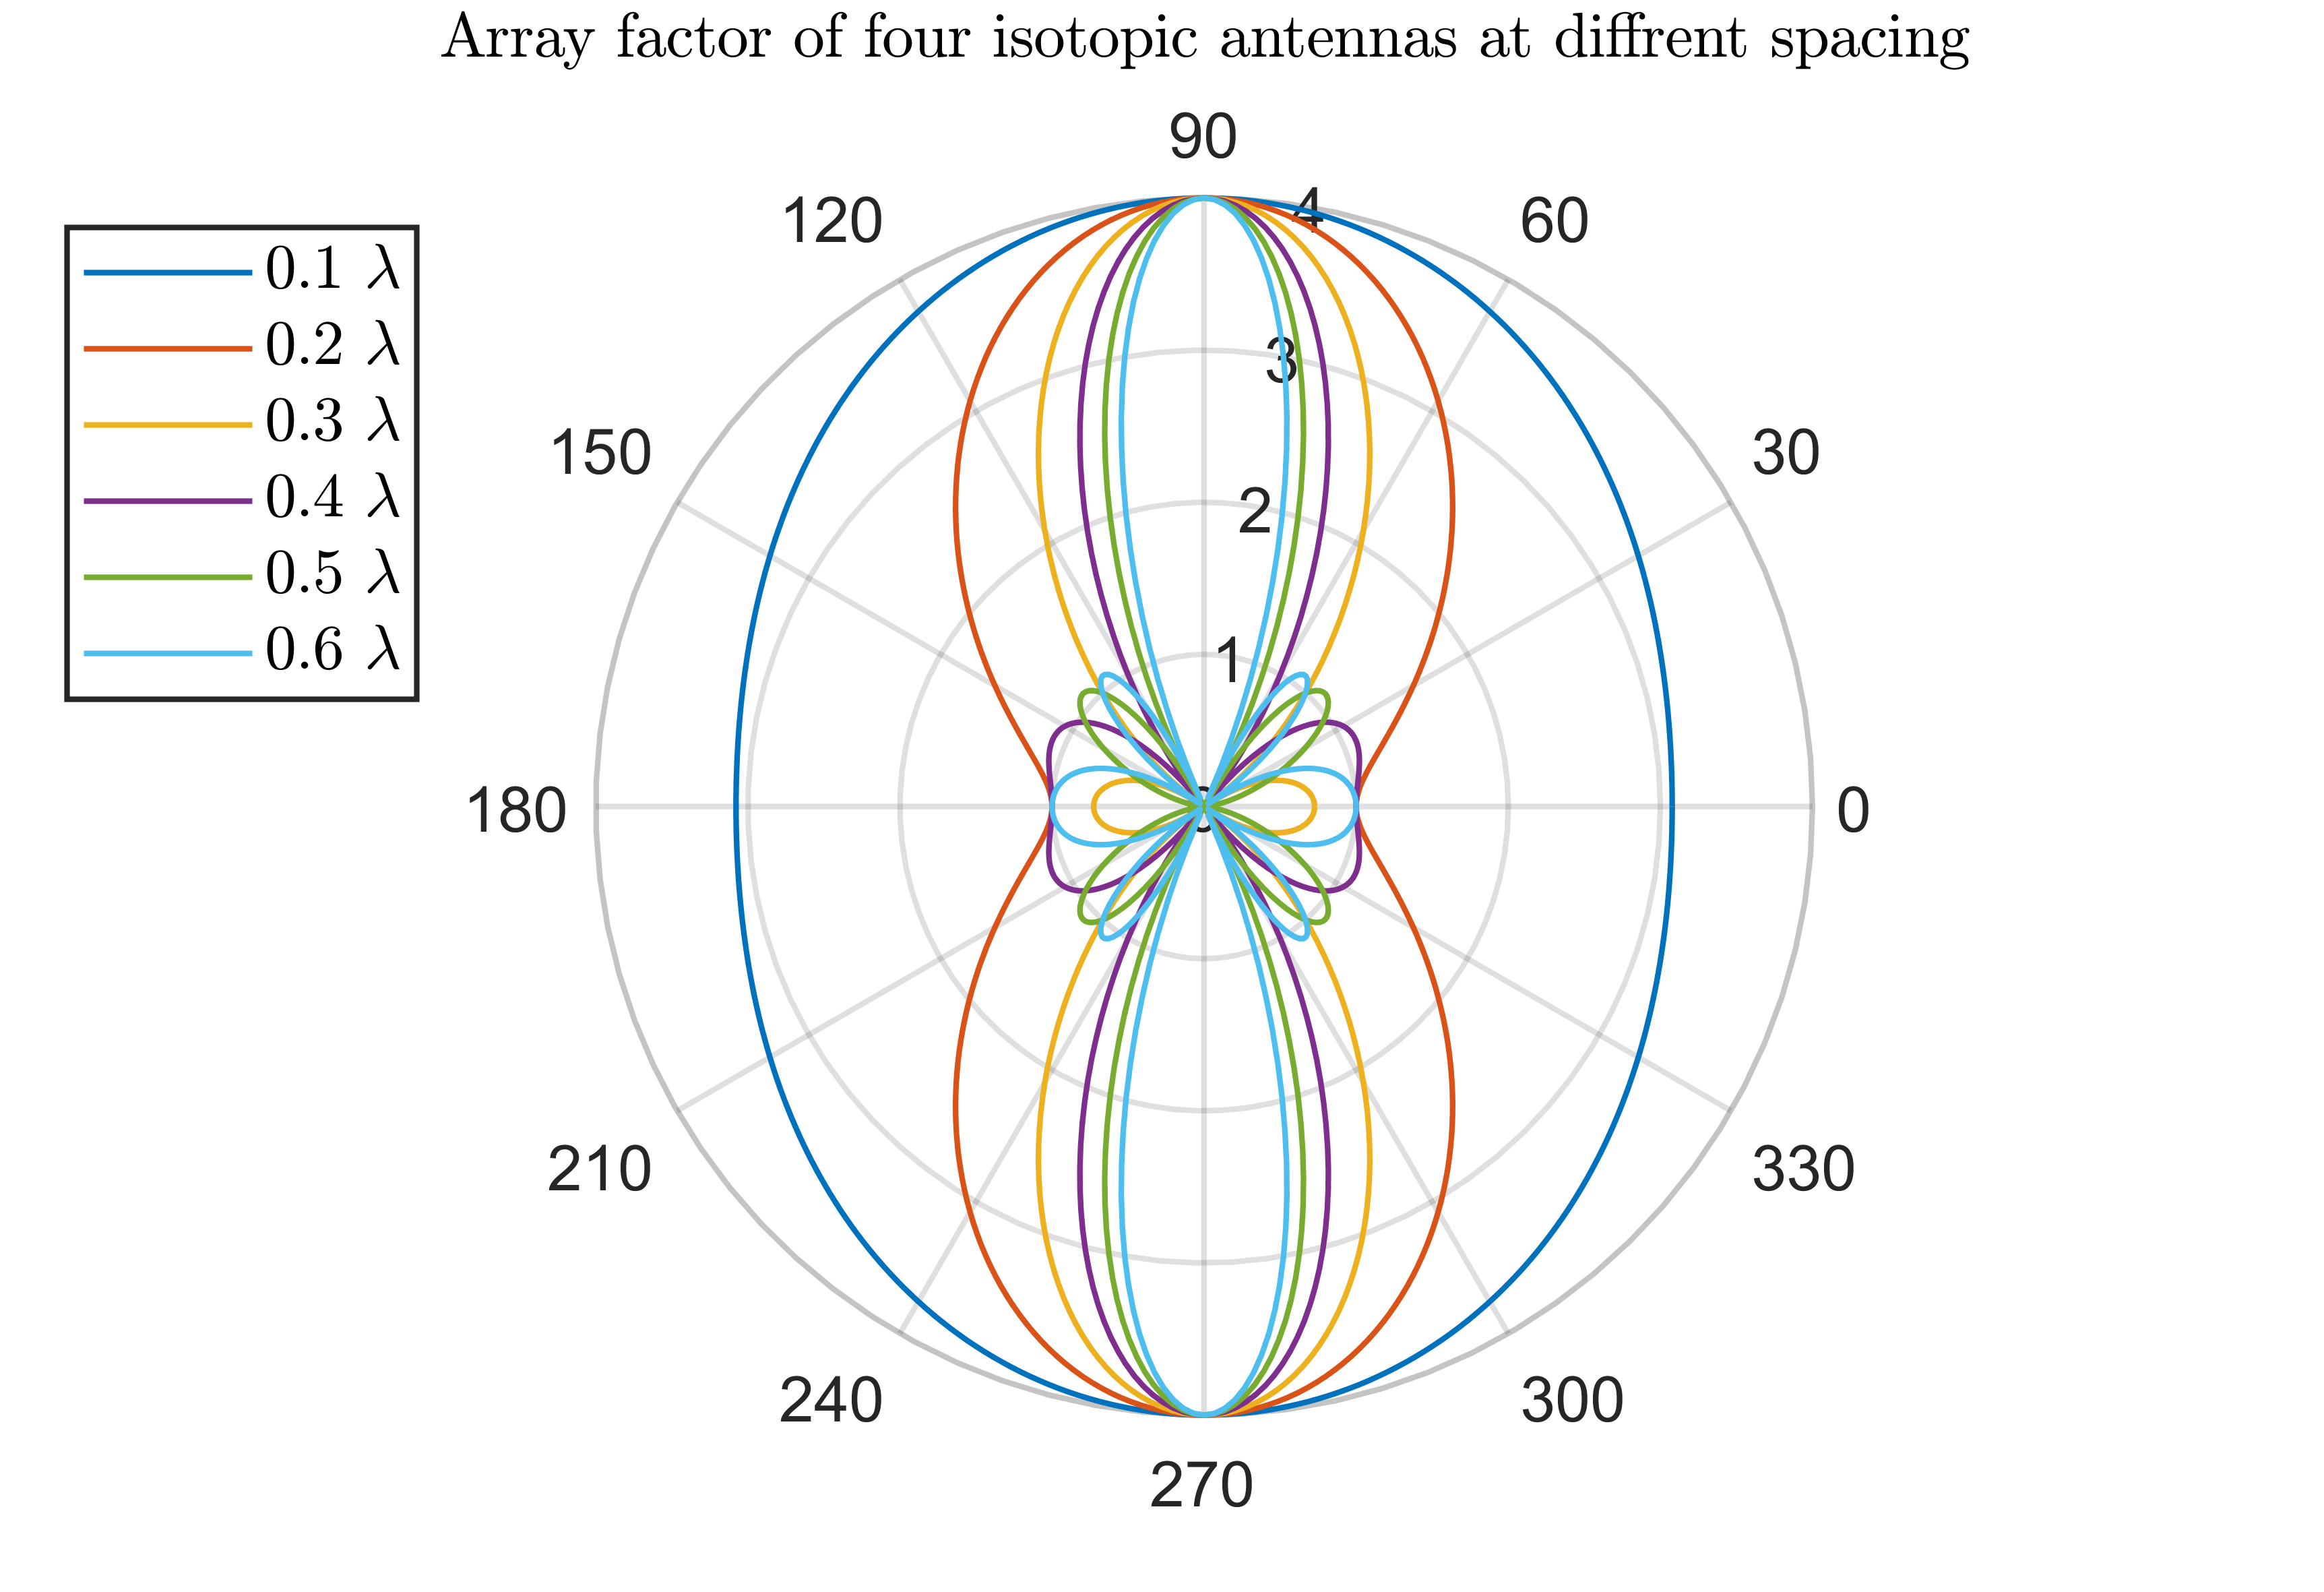
\includegraphics[scale = 0.7]{figures/measurement/af_4ant.png}
\caption{Array factor of four antennas with diffrent spacing}
\label{fig:af_4ant}
\end{figure}







\chapter{Conclusion}\label{ch:conclusion}
The purpose of this project was to investigate the effects from crosstalk at antenna arrays connected to PAs when they are linearised with DPD. It was shown that it is not necessary to include a mathematical model for the antenna if only one antenna is used at a single amplifier. It was further shown that when introducing two amplifiers with one antenna each the conventional DPD technique was not able to compensate for the crosstalk in the antennas. It was therefore tested to measure the setup as a hole and do DPD with the antennas included into the DPD model. This provided better results with a ACPR about 2dB better. When four amplifiers with one antenna each was introduced the technique still lowers the ACPR with 2dB over all distances between the elements in the antenna array. It was also seen from the AM/AM plots that the DPD model was overcompensating at high power-levels. Therfore the proposed model in figure \ref{fig:dpd_pdpd} is shown to be better than conventional DPD, but that there still are space left to improvements. The measurement in section \ref{ch:ant_meas} of the antennas showed a large variation in the S-parameters due to the spacing of the antenna elements. It was also measured if it had any impact that the amplifiers was biased with same bias voltage but different current due to transistor deviations. It was showed that it had little or no impact on the ACPR when treating the amplifiers with antennas as a hole.     




\bibliography{bib/mybib}
\label{bib:mybiblio}
\appendix
\chapter{Antenna measurements}\label{ch:appAlabel}


\end{document}
